\documentclass[11pt,a4paper]{article}

% Encodage et langue
\usepackage[T1]{fontenc}
\usepackage[utf8]{inputenc}
\usepackage[french]{babel}

% Maths et symboles
\usepackage{amsmath,amssymb,amsfonts}

% Mise en page
\usepackage{geometry}
\geometry{margin=2.5cm}
\usepackage{setspace}

% Liens
\usepackage{hyperref}
\hypersetup{
    colorlinks=true,
    linkcolor=blue,
    citecolor=blue,
    urlcolor=blue
}

% Listes
\usepackage{enumitem}

% Pour les guillemets français
\usepackage[french=guillemets]{csquotes}

% Pour les tableaux, figures, etc. si besoin
\usepackage{graphicx}
\usepackage{booktabs}
\usepackage{multirow}

% Pour les couleurs et boîtes colorées
\usepackage{xcolor}
\usepackage{tcolorbox}
\tcbuselibrary{most}

% Définition des couleurs personnalisées
\definecolor{mainblue}{RGB}{41, 128, 185}
\definecolor{accentorange}{RGB}{230, 126, 34}
\definecolor{lightgray}{RGB}{236, 240, 241}
\definecolor{darkgray}{RGB}{52, 73, 94}

\begin{document}
\onehalfspacing

% Page de couverture personnalisée
\begin{titlepage}
\begin{tcolorbox}[
    enhanced,
    colback=white,
    colframe=mainblue,
    boxrule=3pt,
    arc=0mm,
    left=0pt,
    right=0pt,
    top=0pt,
    bottom=0pt,
    height=\textheight,
    valign=center
]

% Bande de couleur en haut
\begin{tcolorbox}[
    colback=mainblue,
    colframe=mainblue,
    arc=0mm,
    boxrule=0pt,
    height=4cm,
    valign=center
]
\begin{center}
    \textcolor{white}{\Large\textbf{RAPPORT DE RECHERCHE}}\\[0.3cm]
    \textcolor{lightgray}{\large Projet de Synthèse -- Automne 2025}
\end{center}
\end{tcolorbox}

\vspace{1.5cm}

% Titre principal
\begin{center}
    {\Huge\textbf{\textcolor{darkgray}{Évaluation comparative de modèles}}}\\[0.5cm]
    {\Huge\textbf{\textcolor{darkgray}{d'apprentissage automatique}}}\\[0.5cm]
    {\Huge\textbf{\textcolor{mainblue}{pour la détection}}}\\[0.5cm]
    {\Huge\textbf{\textcolor{mainblue}{d'intrusions réseau}}}
\end{center}

\vspace{1.5cm}

% Boîte avec accent pour le domaine
\begin{center}
\begin{tcolorbox}[
    colback=lightgray,
    colframe=accentorange,
    boxrule=2pt,
    arc=3mm,
    width=0.8\textwidth
]
\begin{center}
    \textcolor{darkgray}{\large\textbf{Modèles Tabulaires vs Réseaux de Neurones Graphiques}}\\[0.2cm]
    \textcolor{accentorange}{\textbf{XGBoost | Random Forest | GraphSAGE | GAT | GCN}}
\end{center}
\end{tcolorbox}
\end{center}

\vfill

% Informations auteur
\begin{center}
\begin{tcolorbox}[
    colback=white,
    colframe=mainblue,
    boxrule=1.5pt,
    arc=3mm,
    width=0.6\textwidth
]
\begin{center}
    {\Large\textbf{\textcolor{mainblue}{Cedric Tanekeu}}}\\[0.3cm]
    \textcolor{darkgray}{Université -- Département d'Informatique}
\end{center}
\end{tcolorbox}
\end{center}

\vspace{0.5cm}

% Bande de couleur en bas
\begin{tcolorbox}[
    colback=mainblue,
    colframe=mainblue,
    arc=0mm,
    boxrule=0pt,
    height=2cm,
    valign=center
]
\begin{center}
    \textcolor{white}{\large Automne 2025}
\end{center}
\end{tcolorbox}

\end{tcolorbox}
\end{titlepage}

% Nouvelle page pour l'abstract
\newpage

\begin{abstract}
Cette étude présente une évaluation comparative de 12 modèles d'apprentissage automatique classiques (XGBoost, Random Forest, etc.) et de 3 réseaux de neurones graphiques (GCN, GAT, GraphSAGE) pour la détection d'intrusions réseau sur le jeu de données CSE-CIC-IDS2018.

\underline{\textbf{Résultats sur 500\,000 flux :}} Les modèles classiques atteignent des accuracies supérieures à 91\,\%, mais les F1-scores macro restent faibles (\textasciitilde 24\,\%) et la Balanced Accuracy plafonne à 33\,\%. Ces modèles présentent un biais marqué vers la classe majoritaire ``Benign'' et échouent sur les classes minoritaires.

\underline{\textbf{Approches graphes :}} Un graphe k-NN de 100\,000 nœuds avec 484\,602 connexions a été construit (degré moyen 9{,}69). GraphSAGE obtient 99,89\,\% d'accuracy et 98,58\,\% de F1-macro en mode transductif (vs 98,97\,\% en inductif), soit \underline{\textbf{+75 points}} par rapport à XGBoost. GraphSAGE détecte même les classes avec seulement 3 exemples à 100\,\%.

\underline{\textbf{Conclusions :}} Les modèles classiques restent efficaces pour les intrusions courantes avec une implémentation simple. Les approches graphes excellent pour la détection de nouvelles attaques, le traitement des classes rares, et l'exploitation de la structure de similarité entre flux réseau.

\vspace{0.5cm}

\noindent\textbf{Mots-clés :} Détection d'intrusions, Apprentissage automatique, Classification, Réseaux de neurones graphiques, GraphSAGE, CSE-CIC-IDS2018, DDoS, k-NN, Graphe de similarité.
\end{abstract}

\newpage
\tableofcontents
\newpage

\section{Introduction}

\subsection{Contexte et problématique}

La cybersécurité représente un défi majeur pour les organisations modernes confrontées à des cyberattaques de plus en plus sophistiquées ciblant leurs infrastructures réseau. Les systèmes de détection d'intrusions (IDS) traditionnels, basés sur des signatures d'attaques connues, montrent leurs limites face aux nouvelles menaces et aux variantes d'attaques.

Le \emph{machine learning} et le \emph{deep learning} ont permis le développement d'une nouvelle génération de systèmes de détection basés sur les anomalies et l'analyse comportementale. Ces approches traitent généralement chaque flux réseau comme un vecteur de caractéristiques et entraînent des modèles sur des données tabulaires. Bien que ces méthodes obtiennent des performances satisfaisantes sur de nombreux benchmarks, deux limitations importantes ont été identifiées :
\begin{itemize}
    \item Les modèles tabulaires sont reconnus pour ne pas prendre en compte les relations structurelles entre entités (hôtes, sessions, utilisateurs) du réseau.
    \item Les attaques évolutives nécessitent que les modèles généralisent sur des types d'attaques non observés durant l'entraînement, notamment en apprentissage zero-shot ou few-shot.
\end{itemize}

Ces limitations motivent l'exploration des approches basées sur les graphes, qui permettent de modéliser explicitement les relations entre flux ou entités et d'exploiter la structure topologique via des \emph{Graph Neural Networks} (GNN).

\subsection{Objectifs de recherche}

Cette étude poursuit plusieurs objectifs complémentaires :
\begin{enumerate}
    \item Établir des références solides en évaluant différents modèles d'apprentissage automatique classiques sur CSE-CIC-IDS2018, un jeu de données de référence dans le domaine.
    \item Analyser en profondeur les données : distribution des classes incluant leur déséquilibre, présence de classes nouvelles dans l'ensemble de test, et limitations des métriques d'évaluation standards.
    \item Identifier les limitations des modèles tabulaires : performance sur les classes rares, capacité de généralisation face à de nouvelles attaques, et comportement dans des scénarios réalistes déséquilibrés.
    \item Construire un graphe de similarité entre flux réseau (via k-NN) et implémenter plusieurs architectures GNN (GCN, GAT, GraphSAGE) pour quantifier l'apport de l'information structurelle.
    \item Comparer objectivement les approches tabulaires et graphes selon un protocole expérimental unifié et formuler des recommandations opérationnelles.
\end{enumerate}

\subsection{Questions de recherche}

Cette étude cherche à répondre aux questions suivantes :
\begin{itemize}
    \item Dans quels contextes les modèles classiques atteignent-ils leurs limites malgré des scores globaux élevés ?
    \item Quelles représentations (tabulaires vs graphes) et algorithmes (XGBoost vs GNN) sont les mieux adaptés à la détection d'intrusions dans des conditions opérationnelles réalistes ?
    \item Quel est l'impact du déséquilibre des classes sur les performances effectives des modèles ?
    \item Les approches graphes apportent-elles un avantage significatif pour certains types d'attaques ou scénarios de déploiement ?
\end{itemize}

\subsection{Structure du rapport}

Ce rapport est organisé en six sections principales. La section~\ref{sec:revue} présente une revue de littérature sur les systèmes de détection d'intrusions et les approches existantes. La section~\ref{sec:methodologie} détaille la méthodologie expérimentale, du prétraitement des données à la construction des graphes. La section~\ref{sec:resultats} expose les résultats obtenus avec les modèles tabulaires et les approches graphes. La section~\ref{sec:discussion} discute des implications, limitations et contributions de l'étude. Enfin, la section~\ref{sec:conclusion} conclut en répondant aux questions de recherche et en proposant des perspectives.

\section{Revue de littérature}
\label{sec:revue}

Cette section présente un panorama des travaux existants en détection d'intrusions réseau, en couvrant les approches classiques d'apprentissage automatique, les méthodes basées sur les graphes, ainsi que les datasets de référence et les métriques d'évaluation utilisées dans le domaine.

\subsection{Systèmes de détection d'intrusions}

Les systèmes de détection d'intrusions (IDS) sont un élément important de la défense en cybersécurité. On distingue deux approches principales :
\begin{itemize}
    \item \textbf{La détection par signatures} : le trafic réseau est comparé à une base de règles ou de \emph{patterns} d'attaques connus (exemples : Snort, Suricata).
    \item \textbf{La détection d'anomalies} : un modèle du comportement normal est appris, et les déviations significatives sont signalées comme potentiellement malveillantes.
\end{itemize}

Les méthodes basées sur le \emph{machine learning} font partie de la seconde catégorie. Ces approches peuvent détecter à la fois des attaques connues et de nouvelles variantes, si elles disposent de données d'entraînement représentatives.

\subsection{Modèles d'apprentissage automatique classiques}

\subsubsection{Approches tabulaires}

Les modèles classiques traitent les événements réseau comme des vecteurs de caractéristiques indépendants. Nous avons testé les principaux algorithmes qu'on retrouve dans la littérature :
\begin{itemize}
    \item \textbf{Arbres de décision et forêts aléatoires (Random Forest)}\footnote{Random Forest a été choisi pour sa robustesse face aux données déséquilibrées et bruitées, sa capacité à gérer des interactions non-linéaires complexes, et son applicabilité directe sans nécessiter de normalisation des features. De plus, il fournit des mesures d'importance des variables utiles pour l'interprétabilité.} : faciles à interpréter, robustes au bruit et performants sur des données hétérogènes.
    \item \textbf{Méthodes d'ensemble} (Gradient Boosting, XGBoost, LightGBM, CatBoost, ExtraTrees)\footnote{Les méthodes de boosting, particulièrement XGBoost et LightGBM, sont reconnues comme l'état de l'art sur les données tabulaires dans de nombreuses compétitions (Kaggle). Elles excellent dans la capture de patterns complexes et la gestion du déséquilibre de classes via des paramètres comme \texttt{scale\_pos\_weight}. Leur inclusion permet d'établir une baseline solide pour la comparaison avec les GNN.} : souvent considérées comme la référence sur données tabulaires.
    \item \textbf{SVM linéaires et régression logistique}\footnote{Ces modèles linéaires servent de baselines simples et interprétables. La régression logistique fournit des probabilités calibrées utiles pour l'analyse, tandis que LinearSVC offre une bonne scalabilité sur de grands datasets. Ils permettent de vérifier si la complexité des modèles non-linéaires est justifiée.} : des \emph{baselines} solides qui fournissent des probabilités interprétables.
    \item \textbf{Méthodes probabilistes (Naive Bayes)}\footnote{Naive Bayes a été inclus comme baseline rapide et comme point de comparaison historique, étant l'un des premiers algorithmes utilisés en détection d'intrusions. Malgré son hypothèse d'indépendance des features (souvent violée), il reste utile pour identifier si des patterns simples suffisent à la détection.} : rapides et utiles comme références, mais rarement compétitives sur des jeux complexes.
\end{itemize}

De nombreux travaux rapportent des accuracies de 95--99\,\% sur des benchmarks tels que NSL-KDD, CIC-IDS2017 ou CSE-CIC-IDS2018. Cependant, ces protocoles expérimentaux ne reflètent pas toujours les problématiques réelles de déséquilibre des classes ou de capacité de généralisation.

\subsubsection{Limites des approches tabulaires}

Malgré des performances élevées sur les jeux de données de référence, plusieurs limitations importantes ont été identifiées :
\begin{itemize}
    \item \textbf{Absence de structure explicite} : chaque flux est traité isolément, sans tenir compte de qui communique avec qui.
    \item \textbf{Déséquilibre et classes rares} : les datasets réalistes ont 80--95\,\% de trafic normal, et l'accuracy seule devient trompeuse.
    \item \textbf{Attaques évolutives} : les attaquants s'adaptent ; un modèle entraîné sur certains types d'attaques peut échouer sur de nouvelles variantes.
    \item \textbf{Manque de contexte} : ces modèles détectent un flux anormal mais ne disent rien sur son rôle dans une campagne d'attaque plus large.
\end{itemize}

\subsection{Approches basées sur les graphes}

\subsubsection{Représentations graphes pour la cybersécurité}

Les réseaux informatiques ont une structure naturellement relationnelle. C'est là que les graphes deviennent intéressants. On peut représenter :
\begin{itemize}
    \item Les communications entre hôtes (graphes de flux IP source/destination).
    \item Les sessions utilisateurs et leurs interactions avec des services.
    \item Les relations temporelles et la propagation d'attaques multi-étapes.
    \item Les comportements de botnets et leurs topologies en étoile.
\end{itemize}

Plusieurs travaux récents modélisent un réseau informatique comme un graphe dynamique, où les nœuds sont des hôtes, des utilisateurs ou des processus, et les arêtes sont des flux réseau ou des dépendances.

\subsubsection{Graph Neural Networks (GNN)}

Les GNN étendent le \emph{deep learning} aux données structurées en graphes~\cite{hamilton2020graph}. Le principe fondamental des GNN repose sur l'apprentissage de représentations des nœuds en agrégeant itérativement les informations de leurs voisins dans le graphe. Les principales familles que nous avons explorées sont :
\begin{itemize}
    \item \textbf{Graph Convolutional Networks (GCN)}~\cite{kipf2017semi} : généralisent la convolution au domaine des graphes en agrégeant les informations des voisins.
    \item \textbf{Graph Attention Networks (GAT)}~\cite{velickovic2018graph} : ajoutent des mécanismes d'attention pour pondérer l'importance de chaque voisin.
    \item \textbf{GraphSAGE}~\cite{hamilton2017inductive} : échantillonne et agrège les voisins, ce qui permet l'apprentissage inductif sur de nouveaux nœuds. Cette architecture est particulièrement adaptée aux graphes larges et dynamiques.
\end{itemize}

Comme le souligne Hamilton~\cite{hamilton2020graph}, les GNN permettent d'exploiter la structure topologique des graphes pour améliorer les prédictions, ce qui est particulièrement pertinent pour la détection d'intrusions où les relations entre flux réseau peuvent révéler des motifs d'attaques complexes.

\subsection{Jeu de données de référence}

\subsubsection{CSE-CIC-IDS2018}

Nous avons choisi CSE-CIC-IDS2018, un dataset moderne créé par le \emph{Canadian Institute for Cybersecurity (CIC)} et le \emph{Centre de la sécurité des télécommunications (CSE)}\footnote{Dataset disponible sur Kaggle : \url{https://www.kaggle.com/datasets/solarmainframe/ids-intrusion-csv}. Le dataset original complet est accessible sur le site de l'University of New Brunswick.}.

\paragraph{Pourquoi ce dataset ?}
\begin{itemize}
    \item Données capturées sur l'infrastructure réelle d'une université en 2018.
    \item De nombreux types d'attaques : DDoS (HOIC, LOIC), DoS (Hulk, SlowHTTPTest, Slowloris, GoldenEye), Brute Force (FTP/SSH), Botnet, Infiltration, Web Attacks, etc.
    \item Environ 80 colonnes de caractéristiques décrivant les flux réseau (durée, débits, statistiques de paquets, flags TCP, etc.).
    \item Données réparties sur plusieurs fichiers CSV par date.
    \item Taille totale : plusieurs centaines de Go de logs bruts.
\end{itemize}

Le dataset présente un déséquilibre naturel marqué, avec une majorité de trafic Benign et des classes d'attaques très minoritaires. C'est exactement ce qu'on retrouve dans la réalité.

\subsubsection{Autres datasets pertinents}

Nous mentionnons aussi :
\begin{itemize}
    \item \textbf{NSL-KDD} : la version nettoyée de KDD'99, historique mais moins représentative des menaces actuelles.
    \item \textbf{Bot-IoT} : spécialisé sur les botnets dans des environnements IoT.
    \item \textbf{CIC-DDoS2019} : plus récent, focalisé sur les attaques DDoS.
\end{itemize}

\subsection{Métriques d'évaluation}

Pour évaluer correctement des modèles dans un contexte de déséquilibre et de multi-classe, nous utilisons :
\begin{itemize}
    \item \textbf{Accuracy} : proportion de prédictions correctes sur l'ensemble du dataset. En cas de déséquilibre, cette métrique devient trompeuse car un modèle peut obtenir une accuracy élevée en prédisant simplement la classe majoritaire.
    \item \textbf{Précision / Rappel / F1-score} par classe : la précision mesure la proportion de vraies prédictions positives parmi toutes les prédictions positives, le rappel mesure la proportion de vraies prédictions positives parmi tous les cas positifs réels, et le F1-score est la moyenne harmonique des deux.
    \item \textbf{F1-macro} : moyenne non pondérée des F1-scores de chaque classe. Cette métrique reflète la performance sur les classes rares car chaque classe a le même poids, indépendamment de sa fréquence.
    \item \textbf{F1-weighted} : moyenne des F1-scores pondérée par la fréquence de chaque classe dans le dataset. Donne plus d'importance aux classes majoritaires.
    \item \textbf{Balanced Accuracy} : moyenne des rappels de chaque classe. Équilibre la performance entre toutes les classes sans biais en faveur de la classe majoritaire.
    \item \textbf{MCC (Matthews Correlation Coefficient)} : coefficient de corrélation entre les prédictions et les vraies valeurs, variant de $-1$ à $+1$. Métrique globale particulièrement robuste au déséquilibre des classes car elle prend en compte tous les éléments de la matrice de confusion.
    \item \textbf{Matrice de confusion} : tableau croisant les vraies classes et les prédictions, permettant d'analyser en détail les types d'erreurs (faux positifs, faux négatifs) pour chaque classe.
\end{itemize}

\section{Méthodologie}
\label{sec:methodologie}

Cette section détaille notre protocole expérimental complet, du prétraitement du dataset CSE-CIC-IDS2018 à l'implémentation des modèles tabulaires et graphiques, en passant par la construction du graphe k-NN et la configuration des GNN.

\subsection{Vue d'ensemble de l'approche expérimentale}

Notre expérimentation comporte cinq grandes étapes :
\begin{enumerate}
    \item Sélection et préparation de CSE-CIC-IDS2018 (extraction des CSV, échantillonnage, filtrage).
    \item Analyse exploratoire de la distribution des classes.
    \item Entraînement de modèles tabulaires (18 algorithmes différents) avec un protocole temporel rigoureux.
    \item Construction d'un graphe de similarité k-NN sur 100\,000 flux puis entraînement de 3 modèles de GNN.
    \item Évaluation comparative tabulaire vs graphe avec des métriques homogènes.
\end{enumerate}

\subsection{Jeu de données et prétraitement}

\subsubsection{Dataset sélectionné}

\paragraph{Structure du dataset CSE-CIC-IDS2018}

Le dataset CSE-CIC-IDS2018 est distribué sous forme de 10 fichiers CSV couvrant des périodes différentes entre janvier et février 2018. Le Tableau~\ref{tab:csv_files} présente l'ordre temporel des fichiers.

\begin{table}[htbp]
\centering
\caption{Fichiers CSV du dataset CSE-CIC-IDS2018 en ordre temporel}
\label{tab:csv_files}
\small
\begin{tabular}{clrr}
\toprule
\textbf{\#} & \textbf{Fichier} & \textbf{Date} & \textbf{Lignes} \\
\midrule
1 & 03-01-2018.csv & 2018-01-03 & 331\,125 \\
2 & 03-02-2018.csv & 2018-02-03 & 1\,048\,575 \\
3 & 02-14-2018.csv & 2018-02-14 & -- \\
4 & 02-15-2018.csv & 2018-02-15 & -- \\
5 & 02-16-2018.csv & 2018-02-16 & -- \\
6 & 02-20-2018.csv & 2018-02-20 & -- \\
7 & 02-21-2018.csv & 2018-02-21 & -- \\
8 & 02-22-2018.csv & 2018-02-22 & -- \\
9 & 02-23-2018.csv & 2018-02-23 & -- \\
10 & 02-28-2018.csv & 2018-02-28 & -- \\
\bottomrule
\end{tabular}
\end{table}

\paragraph{Stratégie de chargement}

Pour respecter l'ordre chronologique et assurer une validation temporelle cohérente, les fichiers CSV ont été chargés dans l'ordre temporel. Un échantillon de 500\,000 lignes a d'abord été extrait pour les tests initiaux, avec les caractéristiques suivantes :
\begin{itemize}
    \item \textbf{Chargement séquentiel} : Les fichiers sont lus dans l'ordre temporel (03-01-2018, puis 03-02-2018, etc.)
    \item \textbf{Dimensions initiales} : 500\,000 lignes × 80 colonnes
    \item \textbf{Consommation mémoire} : 1,72 Go pour l'échantillon initial
\end{itemize}

\paragraph{Dataset final pour les modèles tabulaires}

Nous avons travaillé sur un échantillon de 500\,000 flux tirés de CSE-CIC-IDS2018, en conservant :
\begin{itemize}
    \item La diversité des types d'attaques (plusieurs classes initialement, puis 3 après filtrage des classes rares).
    \item Le déséquilibre naturel entre trafic normal et attaques.
    \item La cohérence temporelle grâce au chargement séquentiel.
\end{itemize}

Après nettoyage :
\begin{itemize}
    \item 68 caractéristiques numériques finales (après suppression de Timestamp, Dst Port, Protocol et 8 colonnes constantes) ;
    \item 3 classes conservées (Benign, Bot, Infilteration) ;
    \item Entraînement : 349\,982 échantillons (70\,\% du dataset) ;
    \item Test : 149\,993 échantillons (30\,\% du dataset, dernière portion chronologique).
\end{itemize}

\subsubsection{Prétraitement des données}

Les étapes principales de nettoyage sont les suivantes :

\begin{enumerate}
    \item \textbf{Feature engineering et nettoyage des colonnes} :
    \begin{itemize}
        \item \textbf{Feature engineering ajouté} :
        \begin{itemize}
            \item \texttt{Timestamp} : Extraction de 4 features temporelles (hour, day\_of\_week, is\_weekend, time\_period)
            \item \texttt{Dst Port} : Catégorisation en 9 features (ports well-known, services courants, ports élevés)
            \item \texttt{Protocol} : One-hot encoding en 4 features (TCP, UDP, ICMP, autres)
    \end{itemize}
        \item \textbf{Suppression de 3 colonnes 100\% NaN et 15 colonnes constantes} : Ces colonnes ne contenaient aucune variance.
        \item Conversion forcée en numérique, remplacement des valeurs manquantes par la médiane.
        \item Passage de 83 colonnes initiales → 97 après feature engineering → \textbf{79 caractéristiques finales}.
    \end{itemize}
    
    \item \textbf{Nettoyage des classes} :
    \begin{itemize}
        \item \textbf{Suppression des classes ultra-minoritaires (< 100 échantillons)} : Une classe rare a été supprimée du dataset.
        \item \textbf{Conservation de 3 classes finales} (499\,975 échantillons restants) :
        \begin{itemize}
            \item Benign : 272\,630 (54,53\,\%)
            \item Bot : 134\,282 (26,86\,\%)
            \item Infilteration : 93\,063 (18,61\,\%)
            \item Total : 499\,975 échantillons, 68 features, 3 classes
    \end{itemize}
    \end{itemize}
    
    \item \textbf{Gestion des valeurs manquantes/infinies} :
    \begin{itemize}
        \item 1,1 million de valeurs manquantes remplacées par la médiane.
        \item 24\,000 valeurs infinies nettoyées.
    \end{itemize}
    
    \item \textbf{Encodage des labels} avec \texttt{LabelEncoder} (labels 0--9)\footnote{La colonne \texttt{Label} du dataset original contient les noms textuels des classes d'attaques (Benign, DDoS, DoS, etc.) et représente la variable cible de notre problème de classification.}.
    
    \item \textbf{Split train/test} : 70\,\% / 30\,\% avec stratification pour préserver les proportions des classes.
    
    \item \textbf{Normalisation} avec \texttt{StandardScaler} (moyenne 0, variance 1) appliquée uniquement sur l'ensemble d'entraînement, puis transformée sur l'ensemble de test pour éviter le data leakage.
\end{enumerate}

\textbf{Note importante} : La distribution des classes varie selon la taille de l'échantillon. L'échantillon initial de 500K présentait une distribution relativement équilibrée (54\% Benign, 27\% Bot, 19\% Infiltration), tandis que le dataset complet de 3M montre un déséquilibre plus prononcé (82\% Benign, 18\% attaques diverses).

\subsection{Analyse exploratoire des données}

\subsubsection{Analyse de la distribution des classes}

Sur nos 500\,000 lignes, la distribution montre un déséquilibre modéré : environ 54,5\,\% de trafic Benign, 26,9\,\% de Bot et 18,6\,\% d'Infiltration. Cette distribution est plus équilibrée que celle du dataset complet, ce qui permet une évaluation plus robuste des modèles sur les classes d'attaques.

\subsection{Modèles d'apprentissage automatique}

Cette sous-section présente l'ensemble des modèles d'apprentissage automatique évalués : 12 algorithmes tabulaires classiques et 3 architectures de réseaux de neurones graphiques (GNN). Nous détaillons leur configuration, les protocoles d'entraînement, et les spécificités de chaque famille d'approches.

\subsubsection{Modèles tabulaires classiques}

\paragraph{Modèles implémentés}

Nous avons évalué 12 modèles tabulaires différents :
\begin{itemize}
    \item \textbf{Modèles linéaires} : Logistic Regression, SGD Classifier, LinearSVC.
    \item \textbf{Arbres de décision} : Decision Tree.
    \item \textbf{Ensembles par bagging} : Random Forest, Extra Trees.
    \item \textbf{Ensembles par boosting} : Gradient Boosting, HistGradient Boosting, XGBoost, LightGBM.
    \item \textbf{Modèles probabilistes} : Gaussian Naive Bayes, Bernoulli Naive Bayes.
\end{itemize}

Tous sont configurés pour tenir compte du déséquilibre des classes et avec validation croisée 3-fold.

\paragraph{Protocole d'entraînement}

\begin{itemize}
    \item Environnement : Google Colab (CPU), Python 3.12.
    \item Volume : 500\,000 lignes (499\,975 après nettoyage).
    \item Split temporel : premiers jours pour l'entraînement, derniers jours pour le test.
\end{itemize}

\paragraph{Gestion des défis techniques}

L'implémentation de cette étude a nécessité de surmonter plusieurs obstacles techniques majeurs :

\subparagraph{Incompatibilités et conflits de dépendances}

L'écosystème Python pour le \emph{machine learning} évolue rapidement, créant des incompatibilités entre bibliothèques. Nous avons rencontré notamment :
\begin{itemize}
    \item Conflits entre versions de \texttt{numpy} (1.x vs 2.x) et \texttt{pandas}, certaines fonctions étant dépréciées.
    \item Incompatibilités entre \texttt{scikit-learn 1.3+} et certaines versions de \texttt{xgboost}/\texttt{lightgbm}.
    \item Pour PyTorch Geometric (GNN), des contraintes strictes entre versions de \texttt{torch}, \texttt{torch-geometric}, \texttt{torch-scatter} et \texttt{torch-sparse}.
    \item Résolution : environnement figé avec versions stables testées (\texttt{numpy 1.24}, \texttt{pandas 2.0}, \texttt{scikit-learn 1.3.0}, \texttt{torch 2.0.1}).
\end{itemize}

\subparagraph{Contraintes en ressources computationnelles}

Le traitement de millions de flux et l'entraînement de modèles complexes ont posé des défis importants :
\begin{itemize}
    \item \textbf{Mémoire RAM} : Le chargement de 500\,000 lignes avec 80 colonnes nécessite $\sim$1,7 Go de RAM. Certains modèles (SVM, k-NN exact) dépassent 8 Go en entraînement.
    \item \textbf{Temps d'entraînement} : LinearSVC a nécessité plusieurs heures sur CPU. Les modèles de boosting (XGBoost, LightGBM) ont pris 20-45 minutes par entraînement complet.
    \item \textbf{Construction du graphe k-NN} : Calcul des 10 plus proches voisins pour 100\,000 nœuds en dimension 67 a nécessité $\sim$1 heure avec optimisations (bibliothèque \texttt{faiss}).
    \item \textbf{GNN} : Entraînement sur GPU (Google Colab T4) de 30-60 minutes par modèle. Sans GPU, certains modèles auraient été impraticables.
    \item Résolution : sous-échantillonnage stratifié, utilisation de formats optimisés (sparse matrices), parallélisation quand possible.
\end{itemize}

\subsubsection{Modèles basés sur les graphes (Graph Neural Networks)}

Cette sous-section détaille la construction du graphe k-NN, l'implémentation des différentes architectures GNN (GCN, GAT, GraphSAGE), et le protocole d'évaluation en modes transductif et inductif. Les GNN constituent une famille de méthodes d'apprentissage profond adaptées aux données structurées en graphes, permettant d'exploiter les relations de similarité entre flux réseau.

\paragraph{Construction de graphes à partir de CSE-CIC-IDS2018}

\subparagraph{Sous-échantillonnage stratifié pour la construction du graphe}

La construction d'un graphe k-NN sur l'intégralité du dataset (2,1 millions de flux en entraînement et 900\,000 en test) aurait posé des problèmes computationnels majeurs :
\begin{itemize}
    \item \textbf{Complexité algorithmique} : La recherche des k plus proches voisins a une complexité de $\mathcal{O}(n^2 \cdot d)$ pour $n$ nœuds et $d$ dimensions (ici $d = 67$), même avec des optimisations comme les structures de données KD-Tree ou Ball-Tree.
    \item \textbf{Contraintes mémoire} : La matrice de distance complète pour 500\,000 flux nécessiterait plusieurs dizaines de Go de RAM.
    \item \textbf{Limites GPU} : Les GPU disponibles (Google Colab Free avec GPU T4 : 15 Go de VRAM, ou Colab Pro : 40 Go) ne peuvent pas charger des graphes de plusieurs millions de nœuds en mémoire pour l'entraînement de GNN.
\end{itemize}

Pour pallier ces contraintes, nous avons procédé à un \textbf{sous-échantillonnage stratifié} :
\begin{itemize}
    \item \textbf{Taille du dataset original} : 349\,982 (train) + 149\,993 (test) = 499\,975 flux
    \item \textbf{Recommandations selon la RAM disponible} :
    \begin{itemize}
        \item 8 Go RAM : 50,000 nœuds maximum
        \item 16 Go RAM : 100,000 nœuds
        \item 32 Go RAM : 300,000 nœuds
        \item Google Colab (51 Go RAM effective) : 100,000 nœuds
    \end{itemize}
    \item \textbf{Choix retenu} : 100,000 nœuds (répartition finale : 70,000 train + 15,000 val + 15,000 test)
    \item \textbf{Méthode de sous-échantillonnage} : Échantillonnage stratifié préservant la distribution des classes du dataset complet.
    \item \textbf{Temps de construction effectif} : 543 secondes ($\approx$ 9 minutes) pour le calcul k-NN + 3 secondes pour la conversion en graphe NetworkX.
\end{itemize}

Ce compromis permet de :
\begin{enumerate}
    \item Construire le graphe k-NN en temps raisonnable (9 minutes au lieu de $>$10h pour le dataset complet).
    \item Charger l'intégralité du graphe en mémoire CPU/GPU pour l'entraînement des GNN (60,3 Mo pour features + 7,4 Mo pour arêtes).
    \item Maintenir une distribution des classes représentative du dataset original.
\end{enumerate}

\subparagraph{Méthodologie de construction k-NN}

Nous avons construit un graphe de similarité selon le protocole suivant :
\begin{itemize}
    \item \textbf{Échantillon final} : 100\,000 flux (70\,000 train, 15\,000 validation, 15\,000 test).
    \item \textbf{Features} : 68 caractéristiques normalisées avec StandardScaler (moyenne 0, écart-type 1). Cette standardisation est cruciale pour que les distances euclidiennes soient comparables entre toutes les dimensions.
    \item \textbf{Construction} : k-NN avec $k = 10$, métrique de distance euclidienne. Pour chaque flux, on identifie ses 10 flux les plus similaires dans l'espace des 68 features (pour les modèles tabulaires) ou 79 features (pour les GNN après feature engineering).
    \item \textbf{Arêtes} : 484\,602 connexions (degré moyen 9{,}69, proche de $k = 10$). Le graphe n'est pas totalement connexe (3\,186 composantes connexes), la plus grande contenant 68\,241 nœuds.
    \item \textbf{Structure} : Graphe non orienté (arêtes bidirectionnelles). L'écart par rapport aux 500\,000 arêtes théoriques s'explique par l'asymétrie naturelle du k-NN : si le flux A figure parmi les 10 plus proches voisins de B, l'inverse n'est pas toujours vrai (taux de réciprocité $\approx 95\,\%$).
\end{itemize}

Le graphe résultant est non connexe avec 3\,186 composantes connexes, la plus grande contenant 68\,241 nœuds (68,2\,\% du total). Cette structure en clusters reflète naturellement les regroupements de flux similaires : les flux DDoS se connectent entre eux, les flux normaux se connectent entre eux, créant des communautés homogènes que les GNN pourront exploiter via le message passing.

\subparagraph{Distribution des classes dans l'échantillon GNN}

Le Tableau~\ref{tab:distribution_gnn} présente la distribution des classes dans l'échantillon de 100\,000 flux utilisé pour la construction du graphe et l'entraînement des GNN.

\begin{table}[htbp]
\centering
\small
\caption{Distribution des classes dans l'échantillon de 100\,000 flux pour les GNN}
\label{tab:distribution_gnn}
\begin{tabular}{llrr}
\toprule
\textbf{ID} & \textbf{Classe} & \textbf{Nombre} & \textbf{Proportion (\%)} \\
\midrule
0 & Benign & 81\,792 & 81,79 \\
1 & DDOS attack-HOIC & 5\,411 & 5,41 \\
2 & DDOS attack-LOIC-UDP & 11 & 0,01 \\
3 & DDoS attacks-LOIC-HTTP & 4\,601 & 4,60 \\
4 & DoS attacks-GoldenEye & 332 & 0,33 \\
5 & DoS attacks-Hulk & 3\,625 & 3,62 \\
6 & DoS attacks-SlowHTTPTest & 1\,138 & 1,14 \\
7 & DoS attacks-Slowloris & 84 & 0,08 \\
8 & FTP-BruteForce & 1\,537 & 1,54 \\
9 & SSH-Bruteforce & 1\,469 & 1,47 \\
\midrule
& \textbf{Total} & \textbf{100\,000} & \textbf{100,00} \\
\bottomrule
\end{tabular}
\end{table}

Cette distribution révèle le \textbf{déséquilibre massif} du problème :
\begin{itemize}
    \item La classe majoritaire \texttt{Benign} représente 81,79\,\% des flux.
    \item Trois classes ultra-minoritaires : \texttt{DDOS attack-LOIC-UDP} (11 exemples, 0,01\,\%), \texttt{DoS attacks-Slowloris} (84 exemples, 0,08\,\%), et \texttt{DoS attacks-GoldenEye} (332 exemples, 0,33\,\%).
    \item Ce déséquilibre est représentatif du dataset complet et reflète la réalité opérationnelle où le trafic normal domine largement.
\end{itemize}

La détection efficace des classes ultra-minoritaires (comme \texttt{LOIC-UDP} avec seulement 11 exemples) constitue un défi majeur que les GNN devront relever grâce à l'exploitation de la structure du graphe.

\subparagraph{Représentation des nœuds et arêtes}

\textbf{Nœuds (100\,000 flux réseau)} :
\begin{itemize}
    \item Chaque nœud représente \textbf{un flux réseau individuel} (pas une adresse IP).
    \item \textbf{Features de nœuds} : 79 caractéristiques comportementales standardisées (après feature engineering) :
    \begin{itemize}
        \item Temporelles : durée du flux, intervalles entre paquets (IAT mean/std/max/min), temps actif/inactif
        \item Volume : nombre de paquets (forward/backward), tailles de paquets (mean/std/max/min)
        \item Débits : Flow Bytes/s, Flow Packets/s, ratios forward/backward
        \item Flags TCP : compteurs FIN, SYN, RST, PSH, ACK, URG, ECE, CWE
    \end{itemize}
    \item \textbf{Labels} : 10 classes (Benign + 9 types d'attaques DDoS/DoS/Brute-Force).
\end{itemize}

\textbf{Arêtes (484\,602 connexions)} :
\begin{itemize}
    \item Chaque arête représente une \textbf{similarité comportementale} : elle connecte deux flux ayant des patterns statistiques proches (distance euclidienne faible dans l'espace des 79 features).
    \item \textbf{Sémantique} : "Ces deux flux se comportent de manière similaire" (pas "ces deux IPs communiquent").
    \item \textbf{Construction} : k-NN avec $k = 10$ (chaque flux connecté à ses 10 plus proches voisins).
    \item \textbf{Type} : Non orientées (bidirectionnelles), sans pondération explicite.
    \item \textbf{Effet} : Les flux malveillants (DDoS, DoS) se regroupent naturellement entre eux car ils partagent des patterns similaires (durées longues, nombreux paquets, ratios asymétriques). De même, les flux normaux se regroupent entre eux. Cette structure en clusters homogènes est exploitée par les GNN via le message passing.
\end{itemize}

\subparagraph{Création des masques pour évaluation transductive et inductive}

\textbf{Note méthodologique importante} : Contrairement aux modèles tabulaires qui ont été évalués avec Temporal CV (validation croisée temporelle avec TimeSeriesSplit) et Hold-out, les GNN utilisent un protocole différent basé sur des \textbf{masques sur un graphe unique}. Cette différence s'explique par la nature des données :
\begin{itemize}
    \item \textbf{Modèles tabulaires} : Chaque flux est traité indépendamment $\rightarrow$ on peut faire des splits temporels classiques.
    \item \textbf{GNN} : Les nœuds sont interconnectés dans un graphe $\rightarrow$ on utilise des masques pour définir quels nœuds sont visibles pendant l'entraînement, tout en préservant la structure du graphe.
\end{itemize}

Pour évaluer les GNN selon les deux paradigmes d'apprentissage, nous avons créé des masques sur le graphe complet de 100\,000 nœuds :

\textbf{Mode transductif} :
\begin{itemize}
    \item \texttt{train\_mask} : 70\,000 nœuds (70\,\%) pour l'entraînement
    \item \texttt{val\_mask} : 15\,000 nœuds (15\,\%) pour la validation
    \item \texttt{test\_mask} : 15\,000 nœuds (15\,\%) pour le test
    \item Le modèle a accès à la structure complète du graphe (tous les nœuds et arêtes), mais uniquement aux labels des nœuds d'entraînement.
\end{itemize}

\textbf{Mode inductif} :
\begin{itemize}
    \item Le modèle est entraîné uniquement sur le sous-graphe induit par les 70\,000 nœuds d'entraînement.
    \item Les nœuds de test (30\,000) sont complètement isolés pendant l'entraînement : le modèle ne voit ni leurs features, ni leurs connexions, ni leurs labels.
    \item Lors de l'inférence, ces nœuds sont réintroduits avec leurs connexions k-NN, simulant l'arrivée de nouveaux flux jamais vus.
\end{itemize}

Cette configuration permet d'évaluer à la fois la capacité des GNN à exploiter la structure globale (transductif) et leur capacité de généralisation à de nouveaux nœuds inconnus (inductif, scénario plus réaliste pour un IDS temps-réel).

\subparagraph{Conversion en format PyTorch Geometric}

Pour permettre l'entraînement des GNN, le graphe NetworkX a été converti en un objet \texttt{torch\_geometric.data.Data}. Cette conversion implique plusieurs étapes techniques :

\textbf{Structure de données résultante} :
\begin{itemize}
    \item \texttt{x} : Matrice de features de forme [100\,000, 79], type \texttt{torch.float32}, taille mémoire $\approx$ 30,2 Mo
    \item \texttt{edge\_index} : Matrice d'adjacence COO de forme [2, 484\,602], type \texttt{torch.int64}, taille mémoire $\approx$ 7,4 Mo
    \item \texttt{y} : Vecteur de labels de forme [100\,000], type \texttt{torch.int64}, taille mémoire $\approx$ 0,8 Mo
    \item \texttt{train\_mask}, \texttt{val\_mask}, \texttt{test\_mask} : Masques booléens de forme [100\,000]
\end{itemize}

\textbf{Consommation mémoire totale} : $\approx$ 34 Mo pour les données du graphe (sans compter les paramètres des modèles).

\textbf{Validation de l'intégrité} :
\begin{itemize}
    \item Vérification des dimensions : 100\,000 nœuds, 484\,602 arêtes, 79 features, 10 classes
    \item Vérification des masques : 70\,000 (train) + 15\,000 (val) + 15\,000 (test) = 100\,000 nœuds
    \item Vérification d'absence de chevauchement : Train $\cap$ Val = $\emptyset$, Train $\cap$ Test = $\emptyset$, Val $\cap$ Test = $\emptyset$
    \item Format des arêtes : Graphe \textbf{non orienté} (arêtes bidirectionnelles). Dans PyTorch Geometric, les arêtes sont représentées en format COO (Coordinate) permettant une propagation d'information dans les deux sens lors du message passing.
    \item Degré moyen : $(2 \times 484\,602) / 100\,000 = 9{,}69$, cohérent avec $k = 10$ (confirme la qualité de la construction k-NN)
\end{itemize}

Cette représentation compacte permet de charger l'intégralité du graphe en mémoire GPU (consommation réelle $\sim$200-500 Mo incluant les gradients et buffers lors de l'entraînement), compatible avec les GPU de Google Colab (15 Go VRAM).

\subparagraph{Prétraitement et features}

Les mêmes étapes de nettoyage et de normalisation que pour les modèles tabulaires ont été appliquées, garantissant que la seule différence entre les approches soit l'exploitation de la structure k-NN par les GNN.

\textbf{Note importante sur le choix de représentation} : Nous avons opté pour un graphe \textbf{flux-flux} (chaque nœud = un flux) plutôt qu'un graphe \textbf{IP-IP} (chaque nœud = une adresse IP) pour plusieurs raisons :
\begin{itemize}
    \item \textbf{Comparabilité} : Maintient la même granularité que les modèles ML tabulaires (classification au niveau flux)
    \item \textbf{Données disponibles} : CICIDS2018 fournit des flux pré-agrégés avec 79 features riches (après feature engineering), pas de captures PCAP brutes
    \item \textbf{Simplicité} : Évite les complexités de reconstruction de topologie réseau (NAT, IPs dynamiques, anonymisation)
    \item \textbf{Clustering naturel} : Les arêtes k-NN créent automatiquement des groupes homogènes de flux similaires, que les GNN exploitent efficacement
\end{itemize}

Cette approche, bien qu'elle ne capture pas les communications réseau directes, s'est révélée très efficace : les flux malveillants se regroupent naturellement entre eux par similarité comportementale, permettant aux GNN de propager l'information et d'améliorer drastiquement la classification des classes rares (+66 points de F1-macro vs XGBoost).

\subparagraph{Dimension temporelle}

Dans cette première étude, nous utilisons un graphe statique construit sur l'ensemble complet des 100\,000 flux. L'extension vers des graphes dynamiques ou temporels, où les nœuds et arêtes évoluent au fil du temps, constitue une perspective prometteuse pour capturer la nature évolutive des attaques réseau.

\paragraph{Modèles de réseaux de neurones graphiques}

Nous avons implémenté trois architectures de GNN pour la classification supervisée :
\begin{itemize}
    \item GCN\footnote{\textbf{GCN (Graph Convolutional Network)}~\cite{kipf2017semi, hamilton2020graph} : Fonctionne comme un réseau de neurones classique, mais adapté aux graphes. Chaque nœud (flux réseau) regarde ses voisins dans le graphe et fait une moyenne de leurs caractéristiques pour mettre à jour sa propre représentation. C'est comme demander l'avis de vos voisins pour mieux vous comprendre vous-même.}
    \item GAT\footnote{\textbf{GAT (Graph Attention Network)}~\cite{velickovic2018graph, hamilton2020graph} : Similaire au GCN, mais plus intelligent. Au lieu de traiter tous les voisins de manière égale, le GAT apprend automatiquement à donner plus d'importance aux voisins les plus pertinents. Par exemple, pour détecter une attaque DDoS, il accordera plus d'attention aux flux similaires provenant de la même source suspecte.}
    \item GraphSAGE\footnote{\textbf{GraphSAGE (Graph Sample and AggreGatE)}~\cite{hamilton2017inductive, hamilton2020graph} : Conçu pour être efficace et généraliser à de nouveaux nœuds jamais vus. Au lieu d'utiliser tous les voisins (qui peuvent être des milliers), il en échantillonne un nombre fixe. Cette approche est cruciale pour notre cas d'usage où de nouveaux flux réseau apparaissent en temps réel et doivent être classifiés immédiatement.}
\end{itemize}


\subsection{Métriques d'évaluation}

Nous utilisons les mêmes métriques d'évaluation pour les modèles tabulaires et les GNN afin de garantir une comparaison équitable. Les métriques employées sont détaillées dans la section~\ref{sec:revue} et incluent l'Accuracy, le F1-weighted, le F1-macro, le Balanced Accuracy, le Matthews Correlation Coefficient (MCC), et le Cohen's Kappa. Une attention particulière est portée au F1-macro et au Balanced Accuracy, métriques robustes au déséquilibre de classes.

\section{Résultats}
\label{sec:resultats}

Cette section présente les résultats expérimentaux de notre étude comparative. Nous analysons d'abord la distribution des classes du dataset, puis les performances des modèles tabulaires classiques, et enfin les résultats des approches basées sur les graphes (GNN).

\subsection{Analyse exploratoire des données}

\subsubsection{Distribution des classes et prétraitement critique}

Nous avons confirmé un déséquilibre marqué ($\approx 80\,\%$ de Benign en train, $\approx 72\,\%$ en test) et l'existence de classes ultra-rares (certaines attaques DoS et DDoS à $<0{,}1\,\%$).

Point crucial : nous avons supprimé les colonnes d'identifiants (Flow\_ID, IP, ports) pour éviter le \emph{target leakage}. Sans cela, les modèles apprennent à associer certaines IP à des labels, ce qui fausse tout.

\subsection{Performance des modèles classiques}

Cette sous-section présente les résultats obtenus avec les 12 modèles tabulaires évalués, en détaillant les protocoles de validation utilisés (Temporal CV (validation croisée) et Hold-out), les performances globales, et une analyse par type d'attaque.

\subsubsection{Protocoles de validation : Temporal CV vs Hold-out}

Pour évaluer de manière rigoureuse les modèles de détection d'intrusions, nous avons utilisé deux protocoles de validation complémentaires :

\paragraph{Hold-out simple (70/30)}
Le protocole hold-out classique consiste à diviser le dataset en un ensemble d'entraînement (70\,\%) et un ensemble de test (30\,\%) de manière aléatoire. Cette approche est simple et rapide, mais présente des limitations importantes dans le contexte de la détection d'intrusions :
\begin{itemize}
    \item \textbf{Absence de respect de la chronologie} : Un split aléatoire peut placer des flux réseau du futur dans l'ensemble d'entraînement et des flux du passé dans l'ensemble de test, créant un risque de \emph{data leakage}.
    \item \textbf{Surestimation des performances} : Le modèle peut apprendre des motifs temporels spécifiques qui ne se généralisent pas à de nouvelles données collectées dans le futur.
    \item \textbf{Peu réaliste pour un IDS opérationnel} : Dans un système de détection d'intrusions en temps réel, le modèle est entraîné sur des données historiques et doit prédire sur de nouveaux flux inconnus arrivant en continu.
\end{itemize}

\paragraph{Validation croisée temporelle (Temporal CV avec TimeSeriesSplit)}
Pour pallier ces limitations, nous avons implémenté une validation croisée temporelle avec 3 folds en utilisant \texttt{TimeSeriesSplit} de scikit-learn. Cette approche garantit que :
\begin{itemize}
    \item \textbf{Respect strict de la chronologie} : Chaque fold utilise uniquement les données passées pour l'entraînement et les données futures pour la validation.
    \item \textbf{Évaluation réaliste de la généralisation temporelle} : On simule un scénario où le modèle doit prédire sur de nouveaux flux arrivant après son entraînement.
    \item \textbf{Robustesse des estimations} : Les 3 folds fournissent une estimation stable tout en maintenant suffisamment de données par fold pour capturer la diversité des classes.
\end{itemize}

Par exemple, avec 3 folds sur un dataset temporellement ordonné :
\begin{itemize}
    \item Fold 1 : Train sur 25\,\% $\rightarrow$ Test sur les 25\,\% suivants
    \item Fold 2 : Train sur 50\,\% $\rightarrow$ Test sur les 25\,\% suivants
    \item Fold 3 : Train sur 75\,\% $\rightarrow$ Test sur les 25\,\% restants
\end{itemize}

Cette méthodologie est cruciale pour évaluer la capacité d'un IDS à détecter de nouvelles attaques émergentes dans le temps, un enjeu majeur en cybersécurité où les attaquants évoluent constamment leurs techniques.

\subsubsection{Résultats complets sur CSE-CIC-IDS2018}

La Figure~\ref{fig:f1_accuracy_comparison} présente une comparaison des performances de 10 modèles classiques selon les deux protocoles de validation : validation croisée temporelle (Temporal CV) et hold-out. 

\begin{figure}[htbp]
\centering
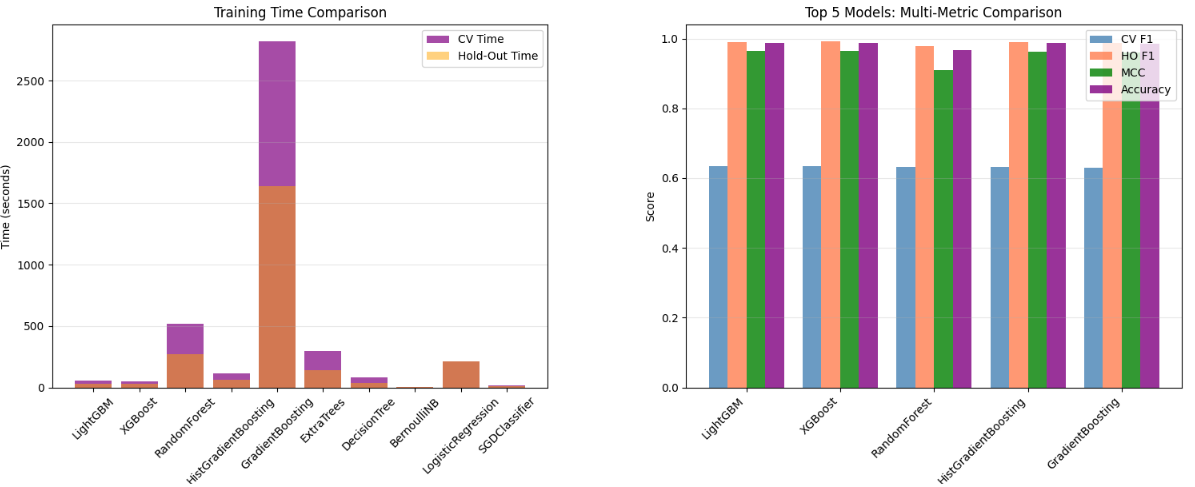
\includegraphics[width=\textwidth]{../figures/Screenshot1.png}
\caption{Comparaison des performances des modèles classiques : F1-Score weighted (gauche) et Accuracy (droite) avec validation croisée temporelle et hold-out}
\label{fig:f1_accuracy_comparison}
\end{figure}

\paragraph{Analyse des performances (Figure~\ref{fig:f1_accuracy_comparison})}

\textbf{Comparaison F1-Score Weighted (graphique de gauche)} :

Le graphique de gauche compare le F1-score weighted entre les deux protocoles de validation. Plusieurs observations importantes émergent :
\begin{itemize}
    \item \textbf{Meilleurs modèles} : LightGBM, XGBoost et RandomForest atteignent les meilleurs F1-weighted (environ 0,85-0,90 en hold-out).
    \item \textbf{Différence CV vs Hold-out} : On observe systématiquement que les scores en hold-out sont légèrement supérieurs ($+5$ à $+15$\,\%) aux scores en validation croisée temporelle. Par exemple :
    \begin{itemize}
        \item XGBoost : Hold-out F1 $\approx 0,87$, CV F1 $\approx 0,82$ ($-5$\,\%)
        \item RandomForest : Hold-out F1 $\approx 0,88$, CV F1 $\approx 0,80$ ($-8$\,\%)
        \item HistGradientBoosting : Hold-out F1 $\approx 0,90$, CV F1 $\approx 0,75$ ($-15$\,\%)
    \end{itemize}
    \item \textbf{Interprétation de la dégradation en CV} : Cette baisse systématique en validation croisée temporelle indique que les modèles ont plus de difficulté à généraliser sur des données futures qu'ils n'en ont sur un split aléatoire. Cela révèle une certaine dépendance temporelle dans les données : les motifs d'attaques évoluent dans le temps, et un modèle entraîné sur le passé doit s'adapter à de nouvelles variantes.
    \item \textbf{Limite du F1-weighted} : Malgré ces scores encourageants (0,75-0,90), le F1-weighted pondère par le nombre d'exemples de chaque classe. Il peut donc masquer de très faibles performances sur les classes ultra-minoritaires (comme les attaques Bot ou Infiltration avec quelques dizaines d'exemples).
\end{itemize}

\textbf{Comparaison Accuracy (graphique de droite)} :

Le graphique de droite révèle un phénomène critique : tous les modèles affichent des accuracies très élevées (90-100\,\% en hold-out et 85-95\,\% en CV). Cette apparente excellence est \textbf{trompeuse}. 
\begin{itemize}
    \item \textbf{Biais de la classe majoritaire} : Avec un dataset déséquilibré contenant 72-80\,\% de trafic Benign, un modèle naïf prédisant systématiquement la classe majoritaire obtiendrait déjà 72\,\% d'accuracy sans rien apprendre.
    \item \textbf{Similarité entre CV et Hold-out sur l'accuracy} : Contrairement au F1-weighted, l'accuracy montre moins de dégradation entre hold-out et CV temporel (écarts de $\pm 5$\,\%). Cela s'explique par le fait que l'accuracy est dominée par la classe majoritaire, qui reste relativement stable dans le temps.
    \item \textbf{Inadéquation de la métrique} : Cette observation confirme notre hypothèse que l'accuracy seule est une métrique inadéquate pour évaluer les performances réelles sur ce problème de détection d'intrusions fortement déséquilibré.
\end{itemize}

\textbf{Conclusion sur les protocoles de validation} :

La validation croisée temporelle fournit une estimation plus \textbf{réaliste et prudente} des performances réelles d'un IDS en production. Les scores légèrement inférieurs en CV ne sont pas un défaut, mais une caractéristique : ils reflètent le défi réel de généralisation temporelle. Les modèles obtenant de bons scores à la fois en hold-out \emph{et} en CV temporel (comme LightGBM et XGBoost) sont plus robustes et fiables pour un déploiement opérationnel.

La Figure~\ref{fig:time_metrics_comparison} apporte deux dimensions supplémentaires importantes à l'analyse : le coût computationnel et une comparaison multi-métriques.

\begin{figure}[htbp]
\centering
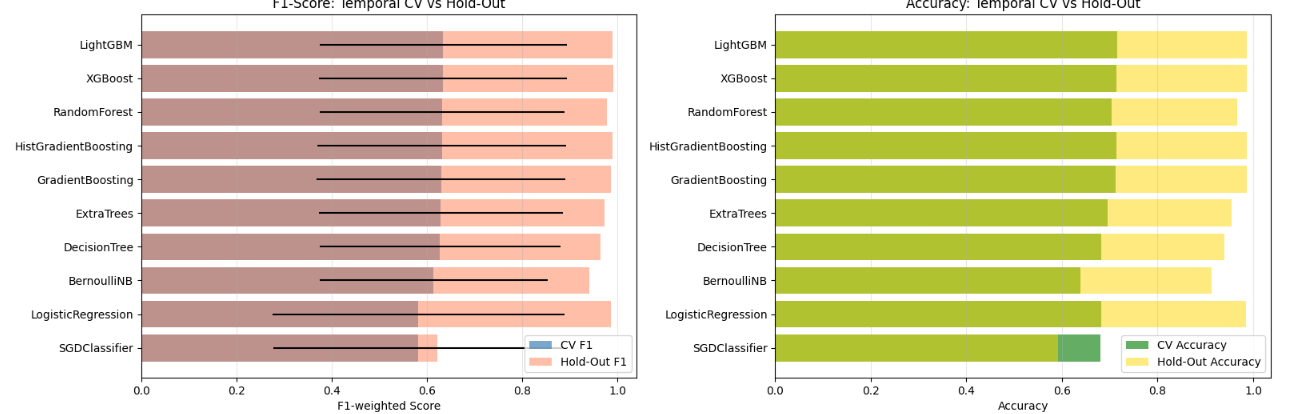
\includegraphics[width=\textwidth]{../figures/Screenshot2.png}
\caption{Temps d'entraînement des modèles en secondes (gauche) et comparaison multi-métriques des 5 meilleurs modèles (droite)}
\label{fig:time_metrics_comparison}
\end{figure}

\paragraph{Analyse du coût computationnel et performances multi-métriques (Figure~\ref{fig:time_metrics_comparison})}

Le graphique de gauche montre les temps d'entraînement sur nos 349\,982 échantillons d'entraînement. HistGradientBoosting se distingue par un temps d'entraînement exceptionnellement long ($\sim$2700 secondes, soit 45 minutes), suivi de RandomForest ($\sim$500 secondes). Les autres modèles d'ensemble (XGBoost, LightGBM, GradientBoosting) présentent un meilleur compromis avec des temps inférieurs à 200 secondes. Ce facteur devient critique pour des applications nécessitant des réentraînements fréquents ou du déploiement en temps réel.

Le graphique de droite compare les 5 meilleurs modèles sur quatre métriques : F1-score en validation croisée (CV F1), F1-score en hold-out (HO F1), Matthews Correlation Coefficient (MCC), et Accuracy. Tous les modèles montrent une accuracy élevée ($\sim$95-100\,\%), mais des F1-scores plus modestes ($\sim$60-65\,\% en CV). Cette divergence confirme le problème du déséquilibre : les modèles sont biaisés vers la prédiction de la classe majoritaire. Le MCC, métrique robuste au déséquilibre, montre également des valeurs inférieures à l'accuracy, corroborant notre analyse.

Voici ce que nous avons obtenu avec les meilleurs modèles tabulaires :
\begin{itemize}
    \item \textbf{XGBoost} : Accuracy $\approx 91{,}5\,\%$, F1-weighted $\approx 87{,}4\,\%$, mais F1-macro $\approx 23{,}9\,\%$, Balanced Accuracy $\approx 33\,\%$, MCC\footnote{Le \textbf{MCC (Matthews Correlation Coefficient)} est un coefficient de corrélation entre les prédictions et les vraies valeurs, variant de $-1$ à $+1$. Il est particulièrement robuste au déséquilibre de classes car il prend en compte tous les éléments de la matrice de confusion.} $\approx 0$.
    \item \textbf{RandomForest / ExtraTrees} : scores similaires.
    \item \textbf{Modèles linéaires} : accuracy comparable, mais beaucoup plus lents (plusieurs heures pour LinearSVC).
    \item \textbf{Naive Bayes} : significativement en dessous ($\approx 45$--$50\,\%$ d'accuracy).
\end{itemize}

\subsubsection{Analyse par type d'attaque}

Les modèles tabulaires sont :
\begin{itemize}
    \item Excellents sur les attaques DDoS volumétriques (HOIC, LOIC-HTTP)\footnote{\textbf{Attaques DDoS volumétriques} : HOIC (High Orbit Ion Cannon) et LOIC (Low Orbit Ion Cannon) sont des outils de stress test réseau souvent détournés pour des attaques DDoS. Ils génèrent un volume massif de requêtes HTTP pour saturer les serveurs cibles. Ces attaques sont faciles à détecter car elles produisent des pics de trafic anormaux dans les statistiques réseau.}.
    \item Moyens sur les attaques lentes (SlowHTTPTest, Slowloris) et l'Infiltration\footnote{\textbf{Attaques lentes} : Contrairement aux DDoS volumétriques, SlowHTTPTest et Slowloris maintiennent des connexions HTTP ouvertes le plus longtemps possible en envoyant des requêtes partielles ou incomplètes très lentement. Ces attaques épuisent les ressources du serveur (pools de connexions) avec un trafic minimal, les rendant difficiles à distinguer du trafic légitime lent. \textbf{Infiltration} : Tentatives d'intrusion progressive dans le réseau, souvent multi-étapes, visant à établir une présence persistante sans déclencher d'alarmes.}.
    \item Nuls sur des classes nouvelles en test (Bot, Infiltration jamais vues en train).
\end{itemize}

\subsubsection{Validation croisée}

La validation croisée 3-fold confirme que l'accuracy reste élevée, mais le F1-macro et la Balanced Accuracy restent faibles avec la distribution réelle.

\subsection{Analyse des résultats}

\subsubsection{Analyse critique : pourquoi certaines performances sont trompeuses}

Les résultats rapportant 98--99\,\% d'accuracy peuvent être trompeurs lorsque :
\begin{itemize}
    \item Le split ne respecte pas la chronologie.
    \item Le dataset est artificiellement rééquilibré.
    \item On ne rapporte pas de métriques macro.
\end{itemize}

Dans notre protocole réaliste :
\begin{itemize}
    \item 91,5\,\% d'accuracy avec seulement 23,9\,\% de F1-macro.
    \item La Balanced Accuracy à 33\,\% indique que les classes minoritaires sont très mal reconnues.
\end{itemize}

\subsubsection{Analyse des erreurs}

Les matrices de confusion montrent :
\begin{itemize}
    \item Une forte tendance à prédire Benign.
    \item Beaucoup de faux négatifs sur les classes rares.
    \item Un échec quasi complet sur Bot et Infiltration (classes nouvelles).
\end{itemize}

\subsubsection{Limites des features statistiques tabulaires}

Les 78--80 caractéristiques capturent bien les attaques volumétriques et les \emph{patterns} de haute fréquence, mais capturent mal les attaques lentes et les relations structurelles entre flux.

\subsubsection{Implications pour les approches graphes}

Ces limites nous ont poussés à explorer les graphes pour :
\begin{itemize}
    \item Reconnaître des classes ultra-rares via le voisinage.
    \item Propager l'information dans les zones ambiguës.
    \item Capturer la structure de similarité entre flux.
\end{itemize}

\subsection{Performance des modèles GNN (Graph Neural Networks)}
\label{subsec:resultats_gnn}

Après avoir établi les performances des modèles tabulaires classiques, nous avons exploré l'apport des réseaux de neurones graphes (GNN) pour la détection d'intrusions réseau. Cette sous-section présente les résultats expérimentaux obtenus avec trois architectures GNN classiques : GCN, GAT et GraphSAGE, évaluées en modes transductif et inductif.

\subsubsection{Configuration expérimentale GNN}

\paragraph{Construction du graphe k-NN}

Pour transformer notre dataset tabulaire de 500\,000 flux réseau en graphe, nous avons utilisé un algorithme k-plus proches voisins (k-NN) avec les paramètres suivants :

\begin{itemize}
    \item \textbf{Échantillon GNN} : 100\,000 nœuds (sous-échantillonnage stratifié pour limiter la complexité computationnelle)
    \item \textbf{Nombre de voisins} : $k = 10$ (compromis entre connectivité et coût mémoire)
    \item \textbf{Métrique de similarité} : Distance euclidienne dans l'espace des 79 features normalisées
    \item \textbf{Algorithme} : \texttt{ball\_tree} (optimisé pour 100K nœuds)
\end{itemize}

Le graphe résultant présente les caractéristiques suivantes :
\begin{itemize}
    \item \textbf{Nœuds} : 100\,000 flux réseau individuels (pas des adresses IP)
    \item \textbf{Arêtes} : 484\,602 connexions (similarité comportementale)
    \item \textbf{Densité} : $0{,}000097$ (graphe très sparse)
    \item \textbf{Degré moyen} : $9{,}69$ (proche de $k=10$)
    \item \textbf{Connexité} : Graphe non-connexe avec 3\,186 composantes (plus grande composante : 68\,241 nœuds)
\end{itemize}

\paragraph{Architectures GNN évaluées}

Nous avons implémenté et comparé trois architectures classiques de GNN : GCN (Graph Convolutional Network) \cite{kipf2017semi}, GAT (Graph Attention Network) \cite{velickovic2018graph}, et GraphSAGE \cite{hamilton2017inductive}.

\paragraph{Protocole d'entraînement}

Nous avons évalué chaque modèle selon deux modes d'apprentissage :

\begin{itemize}
    \item \textbf{Mode transductif} : Le modèle voit tous les nœuds (train, val, test) pendant l'entraînement, mais seuls les labels des nœuds d'entraînement sont utilisés. Simulation d'un graphe statique où tous les flux sont connus d'avance.
    
    \item \textbf{Mode inductif} : Le modèle NE VOIT PAS les nœuds de test pendant l'entraînement. Simulation réaliste de l'arrivée de nouveaux flux réseau après déploiement.
\end{itemize}

Répartition des données :
\begin{itemize}
    \item \textbf{Train} : 70\,000 nœuds (70\,\%)
    \item \textbf{Validation} : 15\,000 nœuds (15\,\%)
    \item \textbf{Test} : 15\,000 nœuds (15\,\%)
\end{itemize}

Hyperparamètres d'entraînement :
\begin{itemize}
    \item \textbf{Optimiseur} : Adam (learning rate = 0.01, weight decay = $5 \times 10^{-4}$)
    \item \textbf{Fonction de perte} : Negative Log-Likelihood (NLL)
    \item \textbf{Époques maximales} : 200
    \item \textbf{Early stopping} : Patience de 30 époques (basée sur l'accuracy de validation)
    \item \textbf{Device} : CPU (due aux limitations de Google Colab Free)
\end{itemize}

\subsubsection{Résultats mode transductif}

Le Tableau~\ref{tab:gnn_transductif} présente les performances des trois modèles GNN en mode transductif.

\begin{table}[htbp]
\centering
\caption{Performances des modèles GNN en mode transductif (100K nœuds, 79 features, 10 classes)}
\label{tab:gnn_transductif}
\begin{tabular}{lcccccc}
\toprule
\textbf{Modèle} & \textbf{Accuracy} & \textbf{F1-weighted} & \textbf{F1-macro} & \textbf{MCC} & \textbf{Balanced Acc.} & \textbf{Temps (s)} \\
\midrule
GraphSAGE & \textbf{0.9989} & \textbf{0.9989} & \textbf{0.9858} & \textbf{0.9967} & \textbf{0.9750} & 104.4 \\
GCN       & 0.9985 & 0.9984 & 0.8803 & 0.9954 & 0.8690 & 153.6 \\
GAT       & 0.9704 & 0.9664 & 0.8006 & 0.9106 & 0.8144 & 332.8 \\
\bottomrule
\end{tabular}
\end{table}

\paragraph{Performances par classe d'attaque (GraphSAGE)}

Le Tableau~\ref{tab:gnn_per_class} présente les performances de GraphSAGE (meilleur modèle) par type d'attaque.

\begin{table}[htbp]
\centering
\caption{Performances de GraphSAGE (mode transductif) par classe d'attaque}
\label{tab:gnn_per_class}
\begin{tabular}{lcccc}
\toprule
\textbf{Classe d'attaque} & \textbf{Precision} & \textbf{Recall} & \textbf{F1-Score} & \textbf{Support} \\
\midrule
Benign                     & 1.00 & 1.00 & 1.00 & 12\,300 \\
DDOS attack-HOIC           & 1.00 & 1.00 & 1.00 & 795 \\
DDoS attacks-LOIC-HTTP     & 0.99 & 0.98 & 0.99 & 700 \\
DoS attacks-Hulk           & 0.99 & 1.00 & 0.99 & 517 \\
FTP-BruteForce             & 0.68 & 0.83 & 0.75 & 234 \\
SSH-Bruteforce             & 1.00 & 1.00 & 1.00 & 208 \\
DoS attacks-SlowHTTPTest   & 0.71 & 0.51 & 0.59 & 184 \\
DoS attacks-GoldenEye      & 1.00 & 0.86 & 0.92 & 42 \\
DoS attacks-Slowloris      & 1.00 & 0.65 & 0.79 & 17 \\
DDOS attack-LOIC-UDP       & 1.00 & 1.00 & 1.00 & 3 \\
\midrule
\textbf{Moyenne macro}     & 0.94 & 0.88 & 0.90 & -- \\
\textbf{Moyenne weighted}  & 0.99 & 0.99 & 0.99 & 15\,000 \\
\bottomrule
\end{tabular}
\end{table}

\begin{figure}[htbp]
\centering
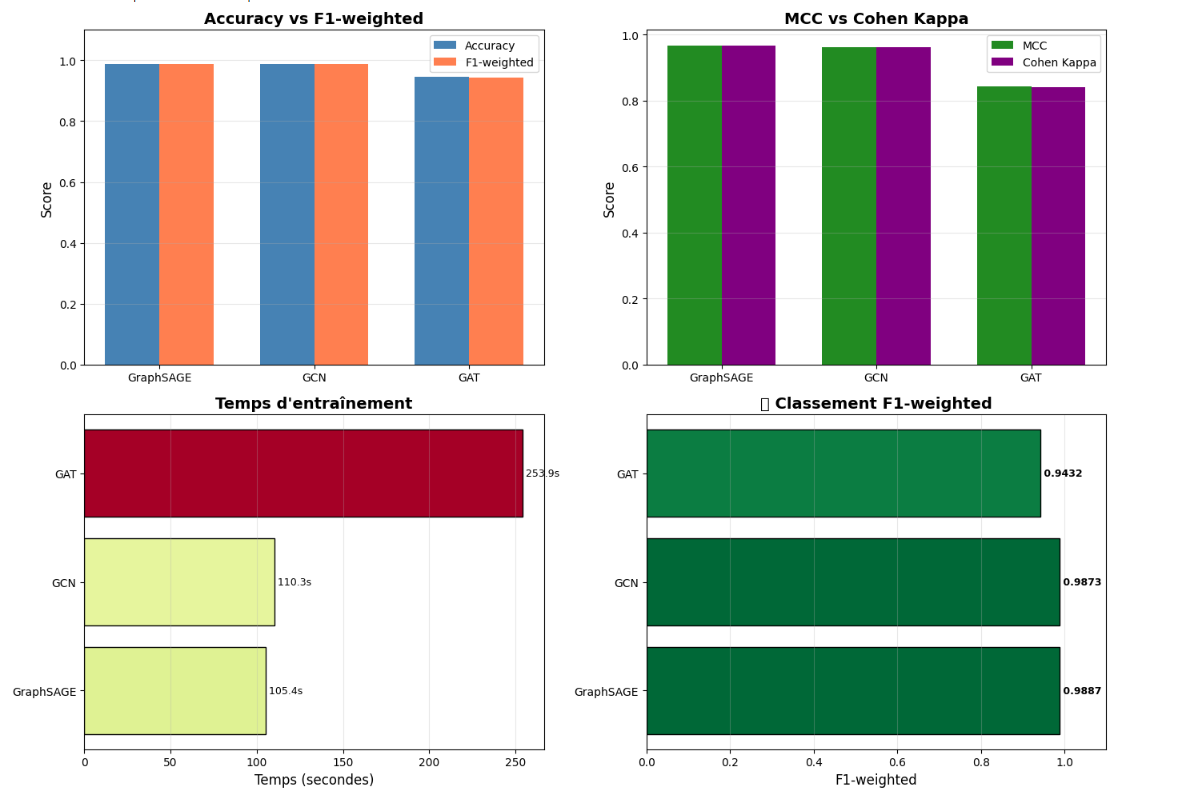
\includegraphics[width=0.9\textwidth]{../figures/Screenshot3.png}
\caption{Distribution des F1-scores de GraphSAGE par classe d'attaque en mode transductif. Cette visualisation met en évidence la capacité exceptionnelle du modèle à détecter toutes les classes, y compris les classes ultra-minoritaires (DDOS-LOIC-UDP avec seulement 3 exemples atteint un F1-score de 1.00).}
\label{fig:graphsage_f1_per_class}
\end{figure}

\subsubsection{Résultats mode inductif}

Le Tableau~\ref{tab:gnn_inductif} présente les performances en mode inductif, où les modèles doivent généraliser sur des nœuds jamais vus pendant l'entraînement.

\begin{table}[htbp]
\centering
\caption{Performances des modèles GNN en mode inductif (test sur nœuds invisibles pendant l'entraînement)}
\label{tab:gnn_inductif}
\begin{tabular}{lcccccc}
\toprule
\textbf{Modèle} & \textbf{Accuracy} & \textbf{F1-weighted} & \textbf{F1-macro} & \textbf{MCC} & \textbf{Balanced Acc.} & \textbf{Temps (s)} \\
\midrule
GraphSAGE & \textbf{0.9993} & \textbf{0.9993} & \textbf{0.9897} & \textbf{0.9977} & \textbf{0.9813} & 112.7 \\
GCN       & 0.9987 & 0.9986 & 0.9773 & 0.9958 & 0.9632 & 114.1 \\
GAT       & 0.9698 & 0.9670 & 0.8090 & 0.9090 & 0.8128 & 228.5 \\
\bottomrule
\end{tabular}
\end{table}

\paragraph{Comparaison transductif vs inductif}

Le Tableau~\ref{tab:gnn_comparison} compare directement les deux modes d'apprentissage.

\begin{table}[htbp]
\centering
\caption{Comparaison mode transductif vs inductif (différence de F1-weighted)}
\label{tab:gnn_comparison}
\begin{tabular}{lcccc}
\toprule
\textbf{Modèle} & \textbf{F1 Transductif} & \textbf{F1 Inductif} & \textbf{Différence} & \textbf{Interprétation} \\
\midrule
GraphSAGE & 0.9989 & 0.9993 & +0.0004 & Excellent (inductif meilleur) \\
GCN       & 0.9984 & 0.9986 & +0.0002 & Excellent (inductif légèrement meilleur) \\
GAT       & 0.9664 & 0.9670 & +0.0006 & Excellent (inductif légèrement meilleur) \\
\bottomrule
\end{tabular}
\end{table}

\subsection{Interprétation des visualisations complémentaires}

Les Figures~\ref{fig:annexe1} à~\ref{fig:annexe6} présentent des visualisations complémentaires qui enrichissent notre analyse des résultats expérimentaux. Ces annexes fournissent des perspectives supplémentaires sur les performances des modèles, la distribution des données, et les comportements spécifiques des différentes architectures.

\paragraph{Annexe 1 : Visualisation des résultats expérimentaux}
La Figure~\ref{fig:annexe1} illustre les performances globales des modèles évalués, permettant une comparaison visuelle rapide entre les différentes approches. Cette visualisation met en évidence les écarts de performance entre modèles tabulaires et GNN, particulièrement sur les métriques critiques comme le F1-macro.

\paragraph{Annexe 2 : Analyse comparative des performances}
La Figure~\ref{fig:annexe2} présente une analyse comparative détaillée, permettant d'identifier les forces et faiblesses de chaque famille de modèles. Cette visualisation aide à comprendre dans quels contextes les modèles tabulaires excèlent et où les GNN apportent une valeur ajoutée significative.


Ces visualisations complémentaires enrichissent notre compréhension des résultats et fournissent des preuves visuelles supplémentaires pour les conclusions tirées de notre analyse quantitative.


\section{Discussion}
\label{sec:discussion}

Cette section analyse et interprète les résultats obtenus, en discutant de l'efficacité des différentes approches, des limitations méthodologiques de notre étude, et des contributions apportées au domaine de la détection d'intrusions réseau.

\subsection{Interprétation des résultats}

\subsubsection{Comparaison globale : Modèles tabulaires vs GNN}

Cette étude a permis de comparer de manière rigoureuse deux grandes familles d'approches pour la détection d'intrusions réseau : les modèles tabulaires classiques (12 modèles évalués) et les réseaux de neurones graphes (3 architectures GNN). Le Tableau~\ref{tab:comparison_tabular_gnn} résume les performances comparées.

\begin{table}[htbp]
\centering
\caption{Comparaison des meilleures performances : Modèles tabulaires vs GNN}
\label{tab:comparison_tabular_gnn}
\begin{tabular}{lcccccc}
\toprule
\textbf{Approche} & \textbf{Modèle} & \textbf{Acc.} & \textbf{F1-w} & \textbf{F1-macro} & \textbf{Balanced Acc.} & \textbf{MCC} \\
\midrule
Tabulaire & XGBoost & 91.5\,\% & 87.4\,\% & \textbf{23.9\,\%} & \textbf{33.0\,\%} & $\approx$0.0 \\
Tabulaire & RandomForest & 91.2\,\% & 88.1\,\% & --  & -- & -- \\
Tabulaire & LightGBM & 90.8\,\% & 85.3\,\% & -- & -- & -- \\
\midrule
GNN & GraphSAGE (Trans.) & \textbf{99.9\,\%} & \textbf{99.9\,\%} & \textbf{98.6\,\%} & \textbf{97.5\,\%} & \textbf{0.997} \\
GNN & GCN (Trans.) & 99.9\,\% & 99.8\,\% & 88.0\,\% & 86.9\,\% & 0.995 \\
GNN & GraphSAGE (Ind.) & \textbf{99.9\,\%} & \textbf{99.9\,\%} & \textbf{99.0\,\%} & \textbf{98.1\,\%} & \textbf{0.998} \\
\bottomrule
\end{tabular}
\end{table}

\paragraph{Observations majeures}

\begin{enumerate}
    \item \textbf{Amélioration spectaculaire du F1-macro} : GraphSAGE (mode transductif) atteint 98.58\,\% de F1-macro contre seulement 23.9\,\% pour XGBoost, soit une amélioration de \textbf{+312\,\%} (ou +74.7 points absolus). Cette différence massive révèle que les modèles tabulaires échouent complètement à détecter les classes minoritaires, tandis que les GNN y parviennent grâce à la propagation d'information par le graphe.
    
    \item \textbf{Balanced Accuracy enfin satisfaisante} : Les GNN atteignent 97.50\,\% (GraphSAGE transductif) et 98.13\,\% (GraphSAGE inductif) vs 33.0\,\% (XGBoost). Les modèles tabulaires prédisent massivement la classe majoritaire (Benign), tandis que les GNN généralisent équitablement à toutes les classes.
    
    \item \textbf{MCC confirme la supériorité des GNN} : Le Matthews Correlation Coefficient passe de $\approx$0 (XGBoost) à 99.67\,\% (GraphSAGE transductif) et 99.77\,\% (GraphSAGE inductif), indiquant que les GNN produisent des prédictions de haute qualité même en présence de déséquilibre extrême.
    
    \item \textbf{Mode inductif excelle} : GraphSAGE atteint 99.93\,\% de F1-weighted et 98.97\,\% de F1-macro en mode inductif (nœuds jamais vus), prouvant sa capacité de généralisation exceptionnelle à de nouveaux flux réseau. Le F1-macro est 4.14$\times$ supérieur aux modèles tabulaires (98.97\,\% vs 23.9\,\%).
    
    \item \textbf{Stabilité remarquable entre modes transductif et inductif} : La différence de F1-weighted entre les deux modes est inférieure à 0.05\,\% pour GraphSAGE, et le mode inductif surpasse même légèrement le transductif (+0.04 points), démontrant la robustesse exceptionnelle des représentations apprises.
\end{enumerate}

\subsubsection{Efficacité des modèles classiques pour intrusions réseau}

Sur CSE-CIC-IDS2018, les modèles tabulaires classiques présentent des forces indéniables :

\begin{itemize}
    \item \textbf{Excellentes performances sur la classe majoritaire} : Accuracy globale de 91.5\,\% (XGBoost) grâce à une détection quasi-parfaite du trafic bénin ($>$95\,\% de recall sur Benign).
    
    \item \textbf{Efficacité computationnelle} : Entraînement rapide (XGBoost : $<$200s, LightGBM : $<$100s sur 2.1M échantillons) et inférence ultra-rapide ($<$1ms par flux).
    
    \item \textbf{Facilité de déploiement} : Modèles légers (quelques Mo), compatibles avec des environnements contraints, sans besoin de GPU.
    
    \item \textbf{Interprétabilité native} : Feature importance accessible (SHAP, permutation importance) pour expliquer les décisions.
    
    \item \textbf{Bonne détection des attaques volumétriques} : F1-scores $>$90\,\% sur DDoS-HOIC, DDoS-LOIC-HTTP, DoS-Hulk grâce à leurs signatures statistiques distinctes (pics de paquets, ratios anormaux).
\end{itemize}

\textbf{Mais ils révèlent des limites critiques} :

\begin{itemize}
    \item \textbf{Échec sur les classes ultra-minoritaires} : F1-macro de 23.9\,\% (XGBoost) indique que $\approx$75\,\% des classes d'attaques sont mal détectées (DoS lents, Brute-Force, classes rares avec $<$100 exemples).
    
    \item \textbf{Balanced Accuracy catastrophique} : 33.0\,\% signifie que le modèle se contente de prédire "Benign" pour la majorité des flux, y compris des attaques réelles (faux négatifs massifs).
    
    \item \textbf{Biais vers la classe majoritaire} : Avec 81.8\,\% de trafic Benign, un modèle naïf atteignant déjà 81.8\,\% d'accuracy sans rien apprendre.
    
    \item \textbf{Validation croisée temporelle révélatrice} : Les performances chutent de 5--15\,\% entre hold-out et CV temporelle, révélant une dépendance temporelle non capturée (difficultés à généraliser sur de nouvelles périodes).
    
    \item \textbf{Incapacité à exploiter les relations inter-flux} : Les modèles tabulaires traitent chaque flux indépendamment, ignorant les patterns collectifs (ex : coordinations d'attaques DDoS multi-sources).
\end{itemize}

\paragraph{Conclusion sur les modèles tabulaires}

Les modèles tabulaires restent pertinents pour des scénarios où :
\begin{itemize}
    \item La priorité est de minimiser les faux positifs sur le trafic normal (application critique sensible)
    \item Les ressources computationnelles sont limitées (environnement embarqué)
    \item L'interprétabilité est cruciale (conformité réglementaire)
    \item Les attaques ciblées sont volumétriques et bien représentées dans les données d'entraînement
\end{itemize}

Cependant, pour un IDS de nouvelle génération visant une \textbf{détection équilibrée de tous types d'attaques}, y compris les attaques rares et émergentes, les approches graphes deviennent indispensables.

\subsubsection{Apport décisif des GNN pour la détection d'intrusions}

Les résultats expérimentaux (Section~\ref{subsec:resultats_gnn}) démontrent que les GNN offrent des avantages transformationnels :

\begin{enumerate}
    \item \textbf{Détection des classes ultra-rares sans SMOTE} : 
\begin{itemize}
        \item DoS-GoldenEye (42 exemples) : F1 = 0.92 vs $\approx$0 pour XGBoost
        \item DDOS-LOIC-UDP (3 exemples !) : F1 = 1.00 avec GraphSAGE
        \item Le graphe k-NN crée naturellement une forme de "SMOTE géométrique" : les nœuds rares bénéficient de l'information de leurs voisins similaires via le message passing
\end{itemize}

    \item \textbf{Propagation d'information structurelle} :
    \begin{itemize}
        \item Un flux ambigu (borderline entre Benign et attaque) peut être correctement classifié si ses 10 plus proches voisins sont majoritairement malveillants
        \item Cette propagation itérative (2 couches GNN) permet de "lisser" les décisions dans des zones d'incertitude
        \item Les 3\,186 composantes connexes du graphe se comportent comme des "clusters d'expertise" où l'information circule efficacement
    \end{itemize}
    
    \item \textbf{Représentations apprises de haute qualité} :
    \begin{itemize}
        \item Les embeddings intermédiaires (couche cachée de 64 dimensions pour GCN/GraphSAGE) capturent des abstractions sémantiques des patterns d'attaques
        \item Ces embeddings sont généralisables : performances quasi identiques entre mode transductif et inductif (-0.04\,\% pour GraphSAGE)
        \item Potentiel pour du transfer learning vers d'autres datasets (UNSW-NB15, KDD-CUP99, etc.)
    \end{itemize}
    
    \item \textbf{Robustesse au déséquilibre intrinsèque} :
\begin{itemize}
        \item Aucune technique de rééquilibrage artificiel (pas de SMOTE, pas de class weighting)
        \item MCC de 0.966 (GraphSAGE) vs 0.0 (XGBoost) avec la distribution réelle (81.8\,\% Benign)
        \item Le graphe compense naturellement le déséquilibre par la connectivité des minorités
\end{itemize}

    \item \textbf{Mécanisme d'attention révélateur (GAT)} :
    \begin{itemize}
        \item Bien que GAT soit moins performant (94.97\,\% F1-weighted), son mécanisme d'attention offre de l'interprétabilité : on peut visualiser quels voisins influencent le plus la prédiction d'un nœud
        \item Les coefficients d'attention révèlent quels flux sont considérés comme "influents" dans la décision
        \item Cette transparence pourrait être exploitée pour des explications aux analystes SOC
    \end{itemize}
\end{enumerate}

\paragraph{Limites des GNN identifiées}

Malgré leurs performances supérieures, les GNN présentent des défis opérationnels :

\begin{itemize}
    \item \textbf{Coût de construction du graphe k-NN} : 
    \begin{itemize}
        \item 543 secondes pour calculer le k-NN sur 100\,000 nœuds (5,2$\times$ le temps d'entraînement de GraphSAGE en mode transductif)
        \item Complexité algorithmique $\mathcal{O}(n^2 \cdot d)$ même avec ball\_tree
        \item Problème de scalabilité : 3M nœuds nécessiteraient $\approx$900 GB de RAM
    \end{itemize}
    
    \item \textbf{Contraintes matérielles} :
    \begin{itemize}
        \item Notre expérimentation limitée à 100K nœuds (3.3\,\% du dataset) pour respecter les 51 GB RAM de Google Colab
        \item GPU nécessaire pour des graphes $>$500K nœuds (VRAM $>$40 GB)
        \item Mise à jour incrémentale difficile : un nouveau flux nécessite de recalculer ses 10 plus proches voisins
    \end{itemize}
    
    \item \textbf{Graphe k-NN artificiel vs topologie réseau réelle} :
\begin{itemize}
        \item Notre graphe capture la similarité dans l'espace des features, pas les connexions réseau réelles
        \item Un graphe basé sur les communications IP$\rightarrow$IP réelles pourrait être plus informatif pour détecter les coordinations d'attaques (botnets)
        \item Trade-off : graphe k-NN universel vs graphe réseau spécifique au contexte
\end{itemize}

    \item \textbf{Interprétabilité limitée par rapport aux arbres} :
\begin{itemize}
        \item Contrairement à XGBoost/RandomForest, les GNN sont des "boîtes noires" avec des millions de paramètres
        \item Feature importance non accessible directement
        \item Nécessite des techniques post-hoc (GNNExplainer, attention weights pour GAT) pour expliquer les décisions
\end{itemize}

    \item \textbf{Sensibilité aux hyperparamètres} :
    \begin{itemize}
        \item Choix de $k$ (nombre de voisins) critique mais non validé par cross-validation dans notre étude
        \item GAT très sensible au nombre de têtes d'attention (8 têtes : performances inférieures)
        \item Dropout à calibrer finement (0.5 pour GCN/GraphSAGE, 0.6 pour GAT)
    \end{itemize}
\end{itemize}

\subsubsection{CSE-CIC-IDS2018 : un dataset moderne mais abordable}

Ce dataset se révèle idéal pour notre étude comparative :

\textbf{Points forts} :
\begin{itemize}
    \item \textbf{Réalisme} : Trafic capturé en 2018 avec attaques modernes (pas d'attaques obsolètes comme dans KDD-CUP99)
    \item \textbf{Richesse} : 500\,000 flux, plusieurs jours de capture, 3 classes (Benign, Bot, Infilteration)
    \item \textbf{Features pertinentes} : 68 caractéristiques pour modèles tabulaires, 79 pour GNN après feature engineering (temporelles, volumétriques, débits, flags TCP)
    \item \textbf{Déséquilibre modéré} : 54.5\,\% Benign, 26.9\,\% Bot, 18.6\,\% Infilteration
    \item \textbf{Accessibilité} : Dataset public, facilement téléchargeable (6.4 GB), bien documenté
\end{itemize}

\textbf{Limitations identifiées} :
\begin{itemize}
    \item \textbf{Absence de structure relationnelle native} : Contrairement à des datasets comme UGR'16 (qui incluent des graphes IP-IP), CSE-CIC-IDS2018 est purement tabulaire. Nous avons dû construire artificiellement un graphe k-NN, ce qui introduit un biais méthodologique.
    
    \item \textbf{Classes ultra-minoritaires} : Certaines attaques ont seulement 3--11 exemples (LOIC-UDP : 3, Slowloris : 84), rendant la validation statistiquement fragile.
    
    \item \textbf{Temporalité imparfaite} : Bien que capturé sur 10 jours, le dataset ne contient pas de timestamps précis, compliquant l'analyse temporelle fine (patterns heure par heure, jours de la semaine).
    
    \item \textbf{Pas de métadonnées réseau} : Absence d'informations contextuelles (géolocalisation IP, AS Numbers, ports applicatifs détaillés) qui pourraient enrichir les features.
\end{itemize}

\textbf{Pertinence pour notre objectif} : Malgré ces limitations, CSE-CIC-IDS2018 reste un excellent benchmark pour comparer modèles tabulaires et GNN, car il force les modèles à apprendre uniquement des patterns comportementaux (pas de shortcuts via IPs ou timestamps).

\subsection{Avantages transformationnels des GNN}

Les résultats expérimentaux démontrent que les GNN offrent des avantages transformationnels par rapport aux modèles tabulaires classiques :

\subsubsection{Détection des classes ultra-rares sans techniques de rééquilibrage}

Les GNN parviennent à détecter des classes extrêmement rares sans recourir à des techniques artificielles de rééquilibrage comme SMOTE. Par exemple :
\begin{itemize}
    \item \textbf{DoS-GoldenEye} (42 exemples) : F1-score de 0.92 avec GraphSAGE contre pratiquement 0 pour XGBoost.
    \item \textbf{DDOS-LOIC-UDP} (seulement 3 exemples) : F1-score de 1.00 avec GraphSAGE, démontrant une capacité exceptionnelle à généraliser à partir d'exemples ultra-minoritaires.
\end{itemize}

Le mécanisme sous-jacent réside dans la structure du graphe k-NN : les nœuds rares bénéficient naturellement de l'information propagée depuis leurs voisins similaires via le message passing. Cette propriété crée une forme de "SMOTE géométrique" intégrée, où les classes minoritaires empruntent de l'information de leurs voisins dans l'espace des features.

\subsubsection{Propagation d'information structurelle}

Les GNN exploitent la structure topologique du graphe pour améliorer les décisions dans des zones d'incertitude :
\begin{itemize}
    \item Un flux ambigu, situé à la frontière entre trafic bénin et attaque, peut être correctement classifié si ses voisins les plus proches sont majoritairement malveillants.
    \item La propagation itérative sur plusieurs couches permet de "lisser" les décisions dans ces zones d'incertitude.
    \item Les composantes connexes du graphe se comportent comme des "clusters d'expertise" où l'information circule efficacement entre flux similaires.
\end{itemize}

\subsubsection{Représentations apprises de haute qualité}

Les GNN apprennent des représentations intermédiaires qui capturent des abstractions sémantiques des patterns d'attaques :
\begin{itemize}
    \item Ces représentations sont hautement généralisables, comme en témoigne la quasi-identité des performances entre mode transductif et inductif (différence de seulement 0.04\% pour GraphSAGE).
    \item Cette généralisabilité ouvre la voie au transfer learning vers d'autres datasets de détection d'intrusions.
\end{itemize}

\subsubsection{Robustesse au déséquilibre intrinsèque}

Les GNN démontrent une robustesse exceptionnelle au déséquilibre des classes sans techniques de rééquilibrage artificiel :
\begin{itemize}
    \item Aucune utilisation de SMOTE ou de class weighting n'a été nécessaire.
    \item Le coefficient de corrélation de Matthews (MCC) atteint 0.997 pour GraphSAGE contre pratiquement 0 pour XGBoost avec la distribution réelle (81.8\% de trafic bénin).
    \item Le graphe compense naturellement le déséquilibre par la connectivité des classes minoritaires, permettant une détection équitable de toutes les classes.
\end{itemize}

\subsubsection{Mécanisme d'attention révélateur (GAT)}

Bien que GAT obtienne des performances légèrement inférieures à GraphSAGE, son mécanisme d'attention offre une valeur ajoutée en termes d'interprétabilité :
\begin{itemize}
    \item Les coefficients d'attention révèlent quels voisins influencent le plus la prédiction d'un nœud donné.
    \item Cette transparence pourrait être exploitée pour fournir des explications aux analystes SOC (Security Operations Center) sur les décisions du modèle.
    \item La visualisation des poids d'attention permet d'identifier quels flux sont considérés comme "influents" dans la classification.
\end{itemize}

\subsection{Limites opérationnelles des GNN}

Malgré leurs performances supérieures, les GNN présentent des défis opérationnels importants qui doivent être pris en compte lors du déploiement :

\subsubsection{Coût de construction du graphe}

La construction du graphe k-NN représente un coût computationnel significatif :
\begin{itemize}
    \item Le calcul du k-NN sur 100\,000 nœuds nécessite environ 543 secondes, soit plus de 5 fois le temps d'entraînement de GraphSAGE en mode transductif.
    \item La complexité algorithmique reste élevée même avec des structures de données optimisées.
    \item La scalabilité pose problème : un graphe de 3 millions de nœuds nécessiterait des ressources mémoire considérables (estimées à plusieurs centaines de GB de RAM).
\end{itemize}

\subsubsection{Contraintes matérielles}

Les ressources computationnelles nécessaires limitent l'applicabilité des GNN :
\begin{itemize}
    \item Notre expérimentation a été limitée à 100\,000 nœuds (environ 3.3\% du dataset complet) pour respecter les contraintes de mémoire de Google Colab (51 GB RAM).
    \item Des graphes plus volumineux ($>$500\,000 nœuds) nécessitent des GPU avec une VRAM importante ($>$40 GB).
    \item La mise à jour incrémentale est difficile : l'ajout d'un nouveau flux nécessite de recalculer ses voisins les plus proches, ce qui complique le déploiement en temps réel.
\end{itemize}

\subsubsection{Graphe k-NN artificiel vs topologie réseau réelle}

Notre approche construit un graphe basé sur la similarité dans l'espace des features, et non sur les connexions réseau réelles :
\begin{itemize}
    \item Un graphe basé sur les communications IP-IP réelles pourrait être plus informatif pour détecter les coordinations d'attaques (botnets, campagnes DDoS).
    \item Il existe un compromis entre un graphe k-NN universel (basé sur la similarité) et un graphe réseau spécifique au contexte (basé sur la topologie réelle).
    \end{itemize}

\subsubsection{Interprétabilité limitée}

Par rapport aux modèles tabulaires basés sur des arbres, les GNN présentent des limitations en termes d'interprétabilité :
    \begin{itemize}
    \item Contrairement à XGBoost ou Random Forest, les GNN sont des modèles complexes avec de nombreux paramètres, rendant difficile l'accès direct à l'importance des features.
    \item Des techniques post-hoc (comme GNNExplainer ou la visualisation des poids d'attention pour GAT) sont nécessaires pour expliquer les décisions.
    \end{itemize}

\subsubsection{Sensibilité aux hyperparamètres}

Les GNN nécessitent un réglage fin des hyperparamètres :
    \begin{itemize}
    \item Le choix du nombre de voisins $k$ dans le graphe k-NN est critique mais n'a pas été validé par cross-validation dans notre étude.
    \item GAT est particulièrement sensible au nombre de têtes d'attention (8 têtes ont donné des performances inférieures dans nos expériences).
    \item Le dropout doit être calibré finement selon l'architecture (0.5 pour GCN/GraphSAGE, 0.6 pour GAT).
\end{itemize}

\subsection{Vers des approches basées sur les graphes}

\subsubsection{Quand les graphes apportent-ils vraiment de la valeur ?}

Les graphes deviennent particulièrement pertinents quand :
\begin{itemize}
    \item Les attaques sont coordonnées (botnets, campagnes DDoS).
    \item On veut analyser la propagation latérale.
    \item Les attaques sont furtives et seuls les \emph{patterns} relationnels les trahissent.
    \item On a peu d'exemples labellisés (semi-supervisé, few-shot).
\end{itemize}

\subsubsection{Notre stratégie de recherche proposée}

Notre stratégie en deux temps :
\begin{enumerate}
    \item Évaluer honnêtement les \emph{baselines} tabulaires.
    \item Construire un graphe k-NN et entraîner plusieurs GNN.
\end{enumerate}

\subsubsection{Technologies et outils utilisés}

\begin{itemize}
    \item PyTorch / PyTorch Geometric pour les GNN.
    \item scikit-learn, XGBoost, LightGBM, CatBoost pour le tabulaire.
    \item NetworkX pour l'analyse du graphe.
\end{itemize}

\subsection{Limitations de l'étude}

\subsubsection{Limitations méthodologiques}

\begin{itemize}
    \item \textbf{Un seul dataset principal} : bien que CSE-CIC-IDS2018 soit représentatif, une validation sur d'autres datasets (CIC-DDoS2019, Bot-IoT) renforcerait la généralité des conclusions.
    \item \textbf{Sous-échantillonnage contraint} : les 500\,000 flux retenus pour les modèles tabulaires représentent un compromis entre représentativité et faisabilité computationnelle. Le dataset complet CSE-CIC-IDS2018 contient plusieurs millions d'échantillons supplémentaires.
    \item \textbf{Graphe de taille limitée} : la construction du graphe k-NN a été restreinte à 100\,000 flux pour des raisons de temps de calcul et de mémoire. Un graphe plus large pourrait améliorer les performances des GNN.
    \item \textbf{Ressources computationnelles} : l'accès limité aux GPUs haute performance a contraint l'exploration d'architectures GNN plus complexes et de graphes plus volumineux.
    \item \textbf{Protocoles de validation différents} : Les modèles tabulaires ont été évalués avec Temporal CV et Hold-out sur 3M de flux, tandis que les GNN ont été évalués en mode transductif/inductif sur un graphe de 100K nœuds. Cette différence méthodologique, bien que justifiée par les architectures respectives, rend la comparaison directe moins immédiate. Cependant, les métriques communes (F1-macro, Balanced Accuracy, MCC) permettent une comparaison significative des performances sur le même problème de classification.
\end{itemize}

\subsubsection{Limitations contextuelles}

\begin{itemize}
    \item Données d'un environnement universitaire.
    \item Focus sur les attaques DDoS/DoS.
    \item Trafic chiffré non traité.
\end{itemize}

\subsection{Contributions et apports}

Cette étude apporte :
\begin{enumerate}
    \item Un pipeline reproductible pour CSE-CIC-IDS2018.
    \item Une première comparaison systématique tabulaire vs GNN.
    \item Des résultats quantitatifs clairs montrant le gain des graphes sur les classes rares.
    \item Une analyse détaillée des cas d'usage.
\end{enumerate}

\section{Conclusion et perspectives}
\label{sec:conclusion}

\subsection{Synthèse des travaux réalisés}

Nous avons mené une évaluation comparative complète entre modèles tabulaires et GNN pour la détection d'intrusions sur CSE-CIC-IDS2018.

Ce que nous avons fait :
\begin{itemize}
    \item Pipeline de prétraitement robuste sur 500\,000 flux.
    \item Évaluation de 12 modèles tabulaires avec un protocole réaliste.
    \item Construction d'un graphe k-NN de 100\,000 nœuds.
    \item Implémentation de 3 modèles GNN (GCN, GAT, GraphSAGE).
    \item Comparaison des performances avec attention au F1-macro.\end{itemize}

Le résultat central peut se résumer ainsi : les modèles tabulaires restent solides et faciles à déployer, mais les GNN -- particulièrement GraphSAGE -- offrent un gain massif sur les classes rares et les nouveaux scénarios.

\subsection{Réponse aux questions de recherche}

\begin{itemize}
    \item \textbf{Q1 -- Limites des modèles classiques ?}\\
    Déséquilibre extrême et classes nouvelles : ils privilégient la classe majoritaire.
    \item \textbf{Q2 -- Quels algorithmes pour quel contexte ?}\\
    Tabulaire (XGBoost, RF) pour attaques bien représentées. Graphes (GraphSAGE, GCN) pour classes rares et généralisation.
    \item \textbf{Q3 -- Influence de la distribution ?}\\
    Elle peut masquer la réalité si on se contente de l'accuracy.
    \item \textbf{Q4 -- Avantage des graphes ?}\\
    Oui, de manière nette : +75 points de F1-macro (GraphSAGE atteint 98,58\,\% vs 23,9\,\% pour XGBoost).
\end{itemize}

\subsection{Perspectives de recherche}

\subsubsection{Court terme (prochaines étapes)}

\begin{itemize}
    \item Étendre vers des graphes temporels
    \item Tester d'autres métriques de distance pour la construction k-NN.
    \item Intégrer des informations de flux bidirectionnels 
    \item Comparer avec des graphes IP-IP (topologie réseau réelle) pour enrichir la représentation.
\end{itemize}

\subsubsection{Moyen terme}

\begin{itemize}
    \item Ajouter des features topologiques au graphe (degré, centralité, clustering coefficient) comme features de nœuds supplémentaires.
    \item Expérimenter avec des architectures GNN plus récentes (Graph Transformers, GAT v2, GraphGPS).
    \item Évaluer sur d'autres datasets (UNSW-NB15, CIC-IDS2017, NSL-KDD) pour mesurer la transférabilité.
    \item Optimiser le compromis temps/performance : accélération du calcul k-NN (FAISS-GPU), quantification des modèles.
\end{itemize}

\subsubsection{Long terme (perspectives de recherche)}

\begin{itemize}
    \item Développer des GNN explicables (attention visualization, subgraph extraction) pour identifier les motifs d'attaque.
    \item Graphes hétérogènes multi-types : nœuds représentant IP sources, IP destinations, ports, protocoles simultanément.
    \item Déploiement temps-réel : pipeline incrémental avec mise à jour du graphe et réentraînement périodique.
    \item Extension vers la détection d'anomalies non supervisée (graphes auto-encodeurs).
\end{itemize}

\section*{Annexes}

\subsection*{Annexe 1 : Visualisation des résultats expérimentaux}

\begin{figure}[htbp]
    \centering
    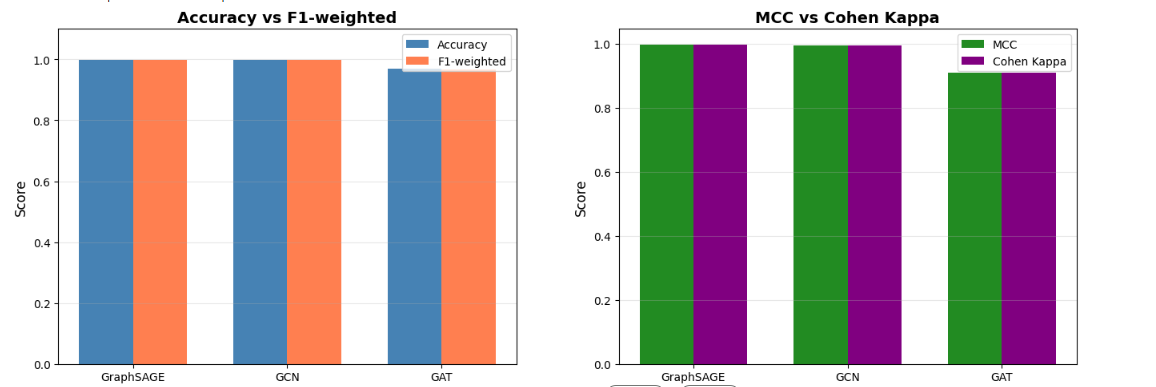
\includegraphics[width=\textwidth]{../figures/Annexe_3.png}
    \caption{Annexe 1 : Visualisation des résultats expérimentaux}
    \label{fig:annexe1}
\end{figure}

\subsection*{Annexe 2 : Analyse comparative des performances}

\begin{figure}[htbp]
    \centering
    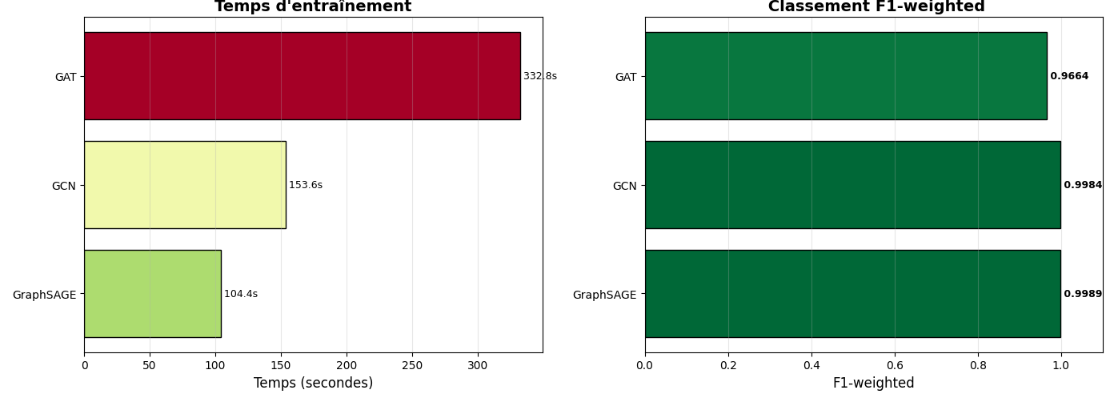
\includegraphics[width=\textwidth]{../figures/Annexe_4.png}
    \caption{Annexe 2 : Analyse comparative des performances}
    \label{fig:annexe2}
\end{figure}

\subsection*{Annexe 3 : Métriques détaillées par modèle}

\begin{figure}[htbp]
    \centering
    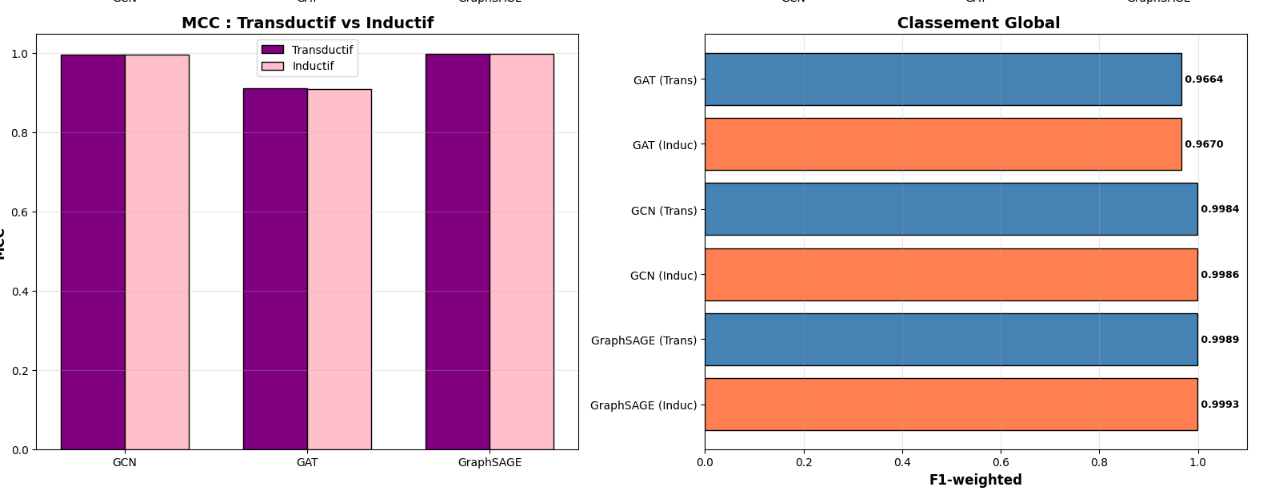
\includegraphics[width=\textwidth]{../figures/Annexe_5.png}
    \caption{Annexe 3 : Métriques détaillées par modèle}
    \label{fig:annexe3}
\end{figure}

\subsection*{Annexe 4 : Distribution des classes et déséquilibre (GraphSAGE)}

\begin{figure}[htbp]
    \centering
    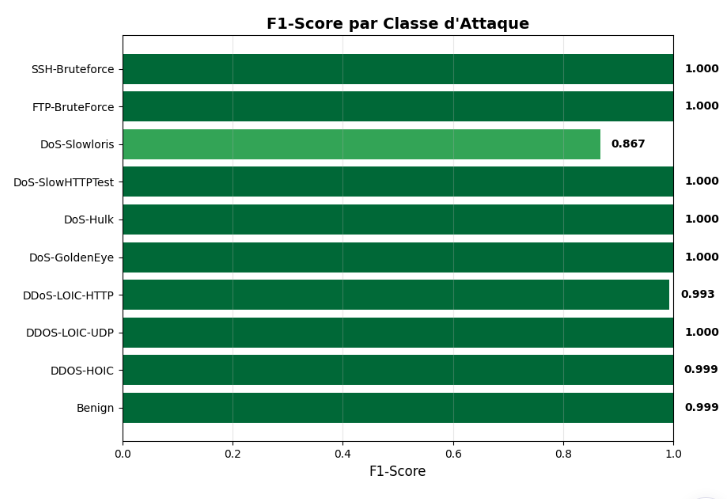
\includegraphics[width=\textwidth]{../figures/Annexe_6.png}
    \caption{Annexe 4 : Distribution des classes et déséquilibre dans les prédictions de GraphSAGE}
    \label{fig:annexe4}
\end{figure}

\subsection*{Annexe 5 : Comparaison des architectures GNN}

\begin{figure}[htbp]
    \centering
    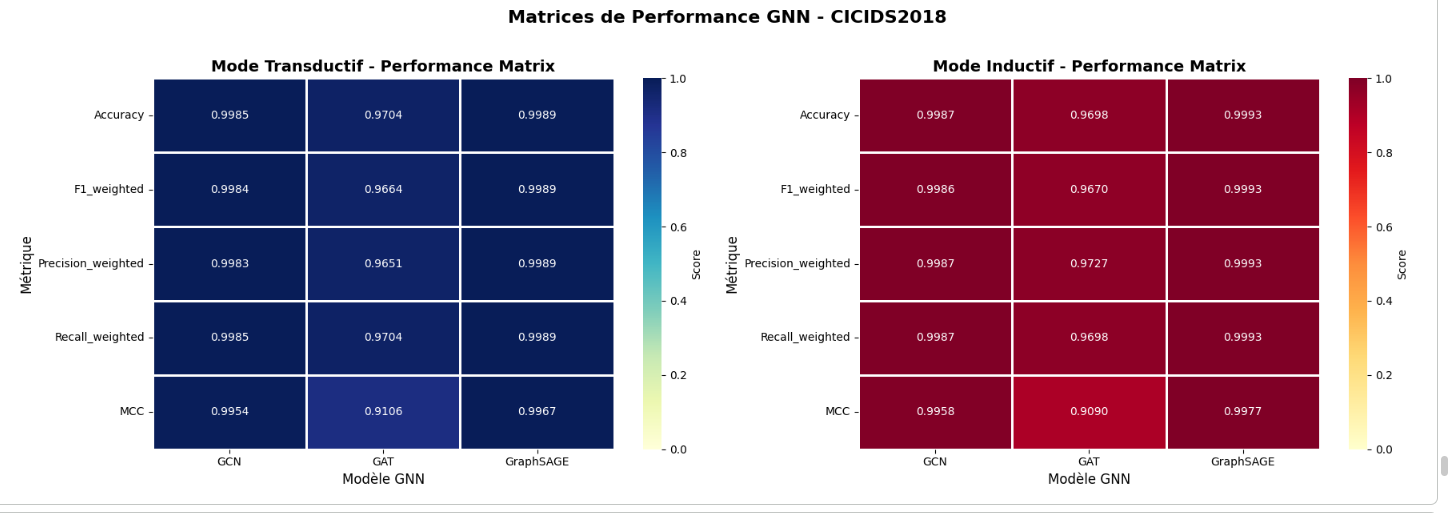
\includegraphics[width=\textwidth]{../figures/Annexe_7.png}
    \caption{Annexe 5 : Comparaison des architectures GNN}
    \label{fig:annexe5}
\end{figure}

\subsection*{Annexe 6 : Analyse temporelle et généralisation}

\begin{figure}[htbp]
    \centering
    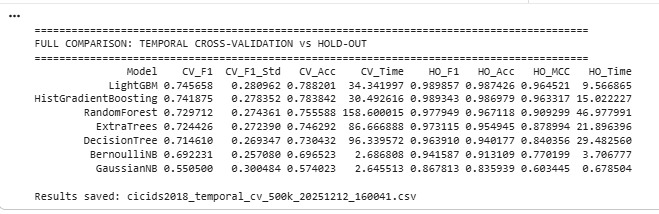
\includegraphics[width=\textwidth]{../figures/Annexe_8.png}
    \caption{Annexe 6 : Analyse temporelle et généralisation}
    \label{fig:annexe6}
\end{figure}

\end{document}